\graphicspath{{2euclid/asy/},{2euclid/pics/}}

\section{Euclidean Geometry}\label{chap:euclid}

\subsection{Euclid's Postulates and Book I of the Elements}\label{sec:euclid}

Euclid's \emph{Elements} (c.\,300\,\BC) formed a core part of European and Islamic curricula until the mid 20\th{} century. Several examples are shown below.
\begin{center}
	\newlength{\heighttt}
	\setlength{\heighttt}{100pt}
	\begin{minipage}[b]{0.35\linewidth}
		\centering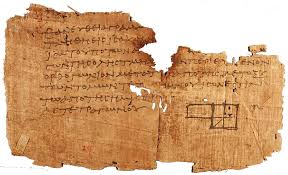
\includegraphics[height=\heighttt]{euclid1}\\
		Earliest Fragment c.\,\AD\,100
	\end{minipage}
	\begin{minipage}[b]{0.3\linewidth}
		\centering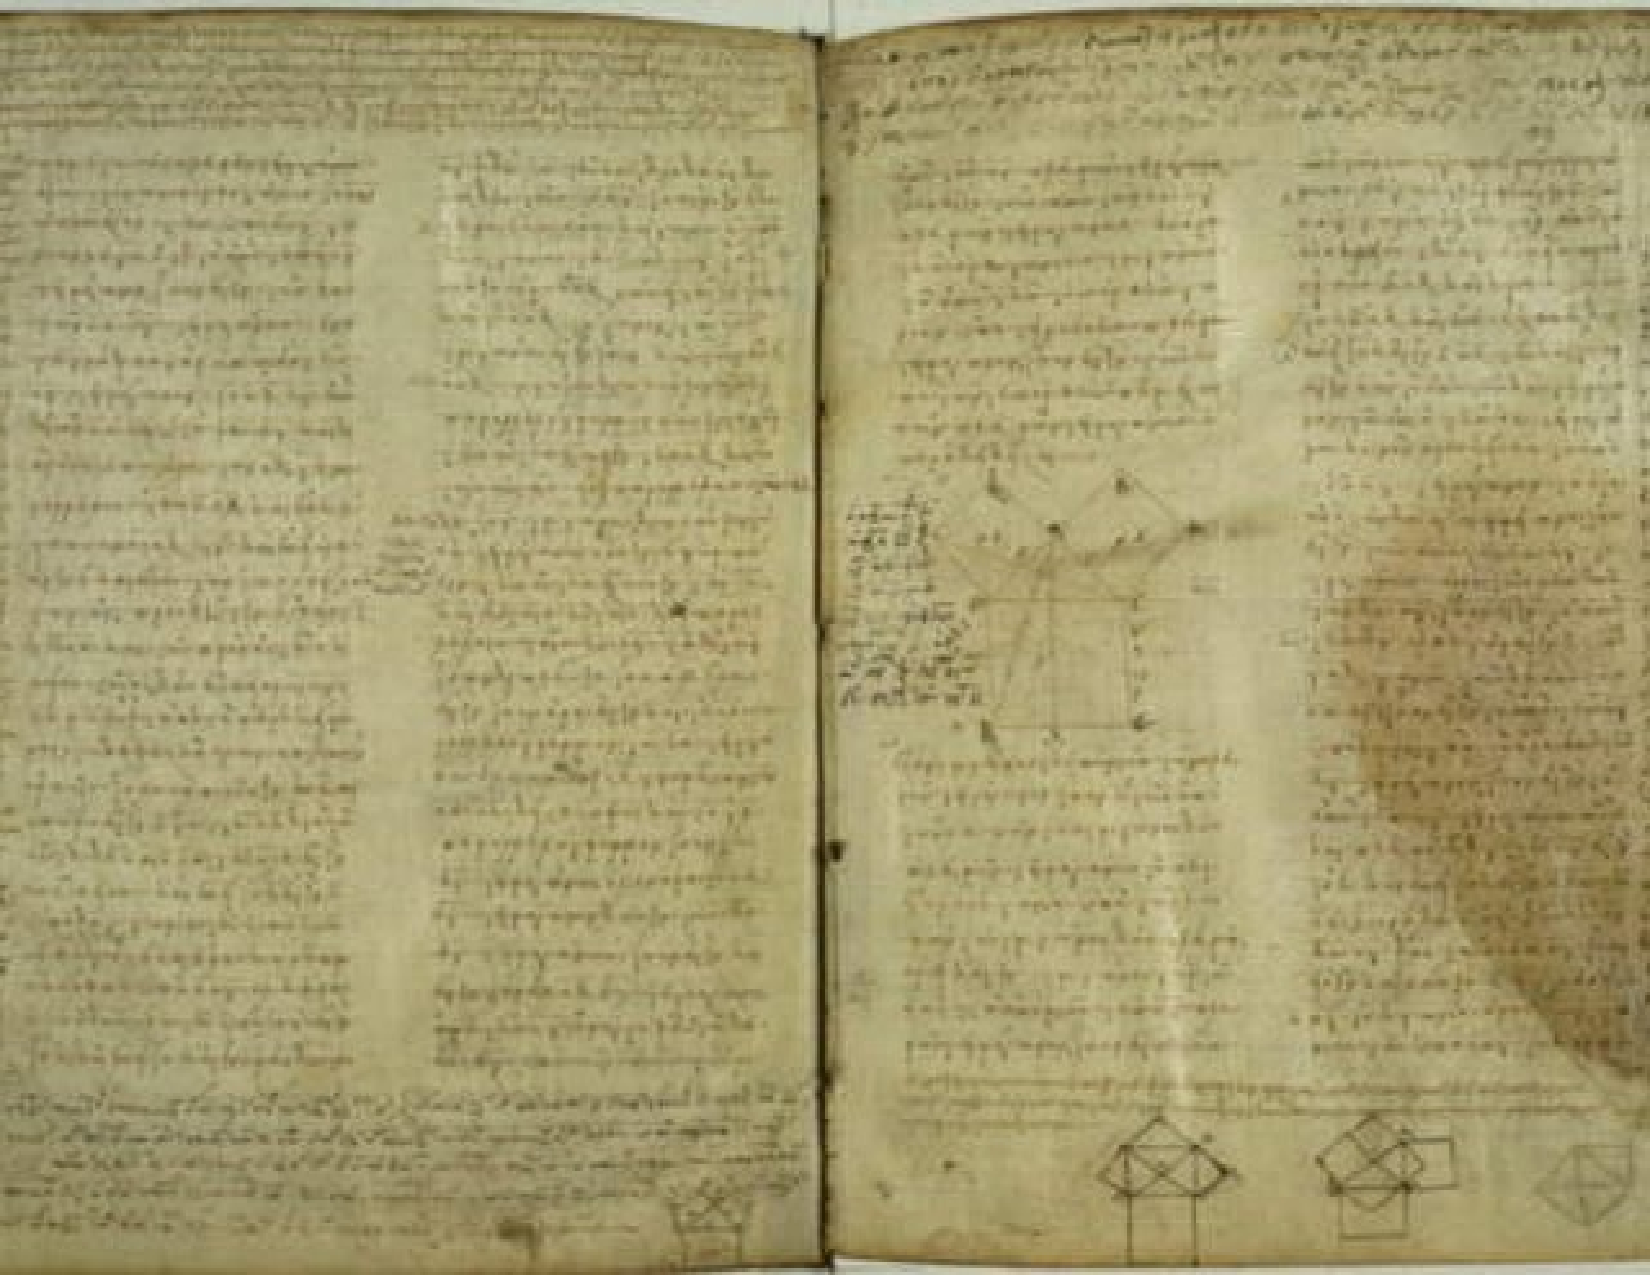
\includegraphics[height=\heighttt]{euclid2}\\
		Full copy, Vatican, 9\th\,C
	\end{minipage}
	\begin{minipage}[b]{0.33\linewidth}
		\centering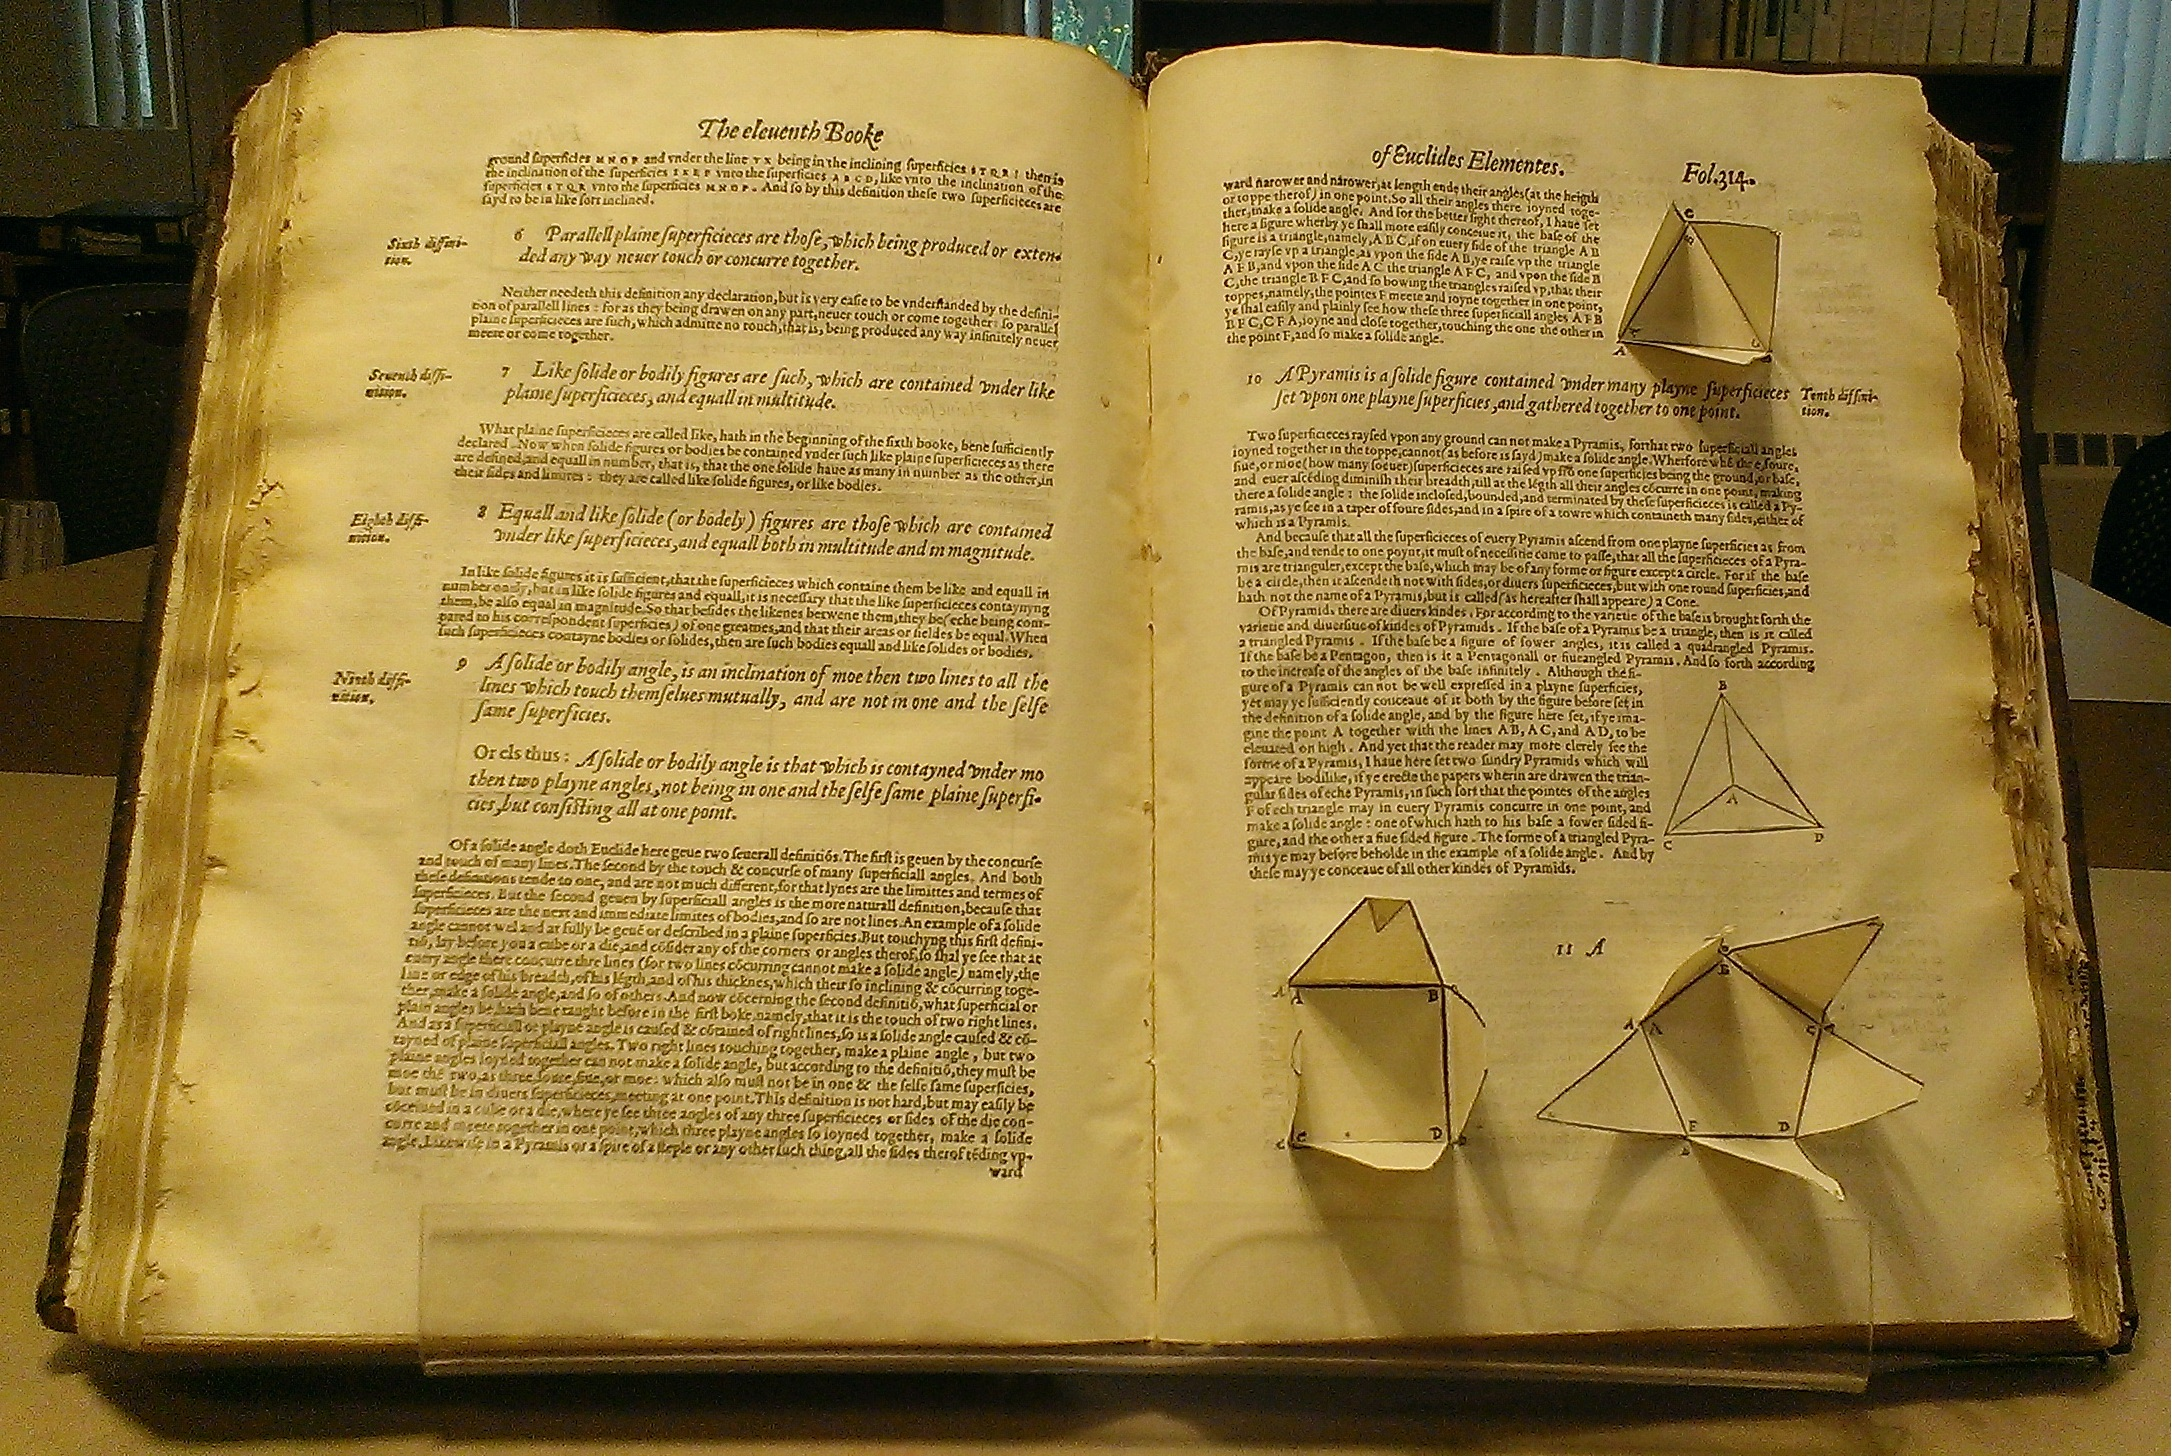
\includegraphics[height=\heighttt]{euclid3}\\
		Pop-up edition, 1500s
	\end{minipage}\\[5pt]
	\setlength{\heighttt}{135pt}
	\begin{minipage}[b]{0.44\linewidth}
		\centering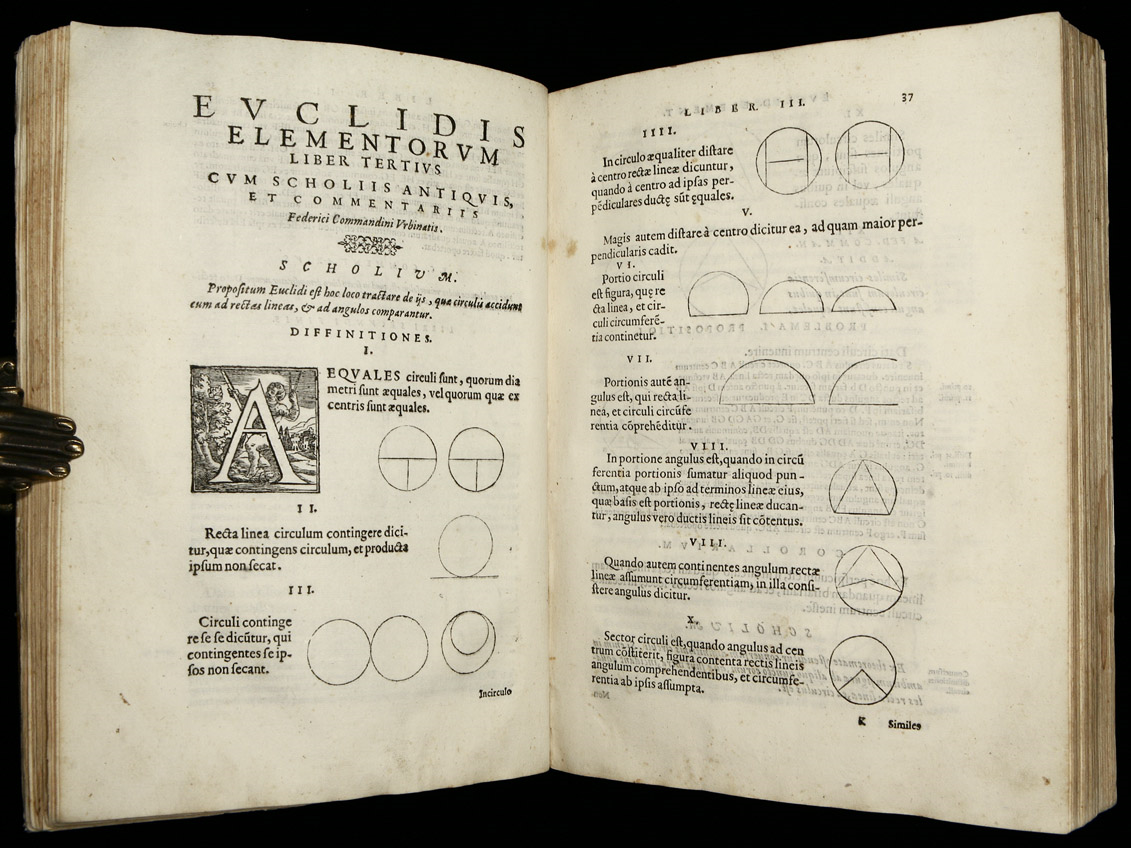
\includegraphics[height=\heighttt]{geo-09-euclid}\\
		Latin translation, 1572
	\end{minipage}
	\begin{minipage}[b]{0.3\linewidth}
		\centering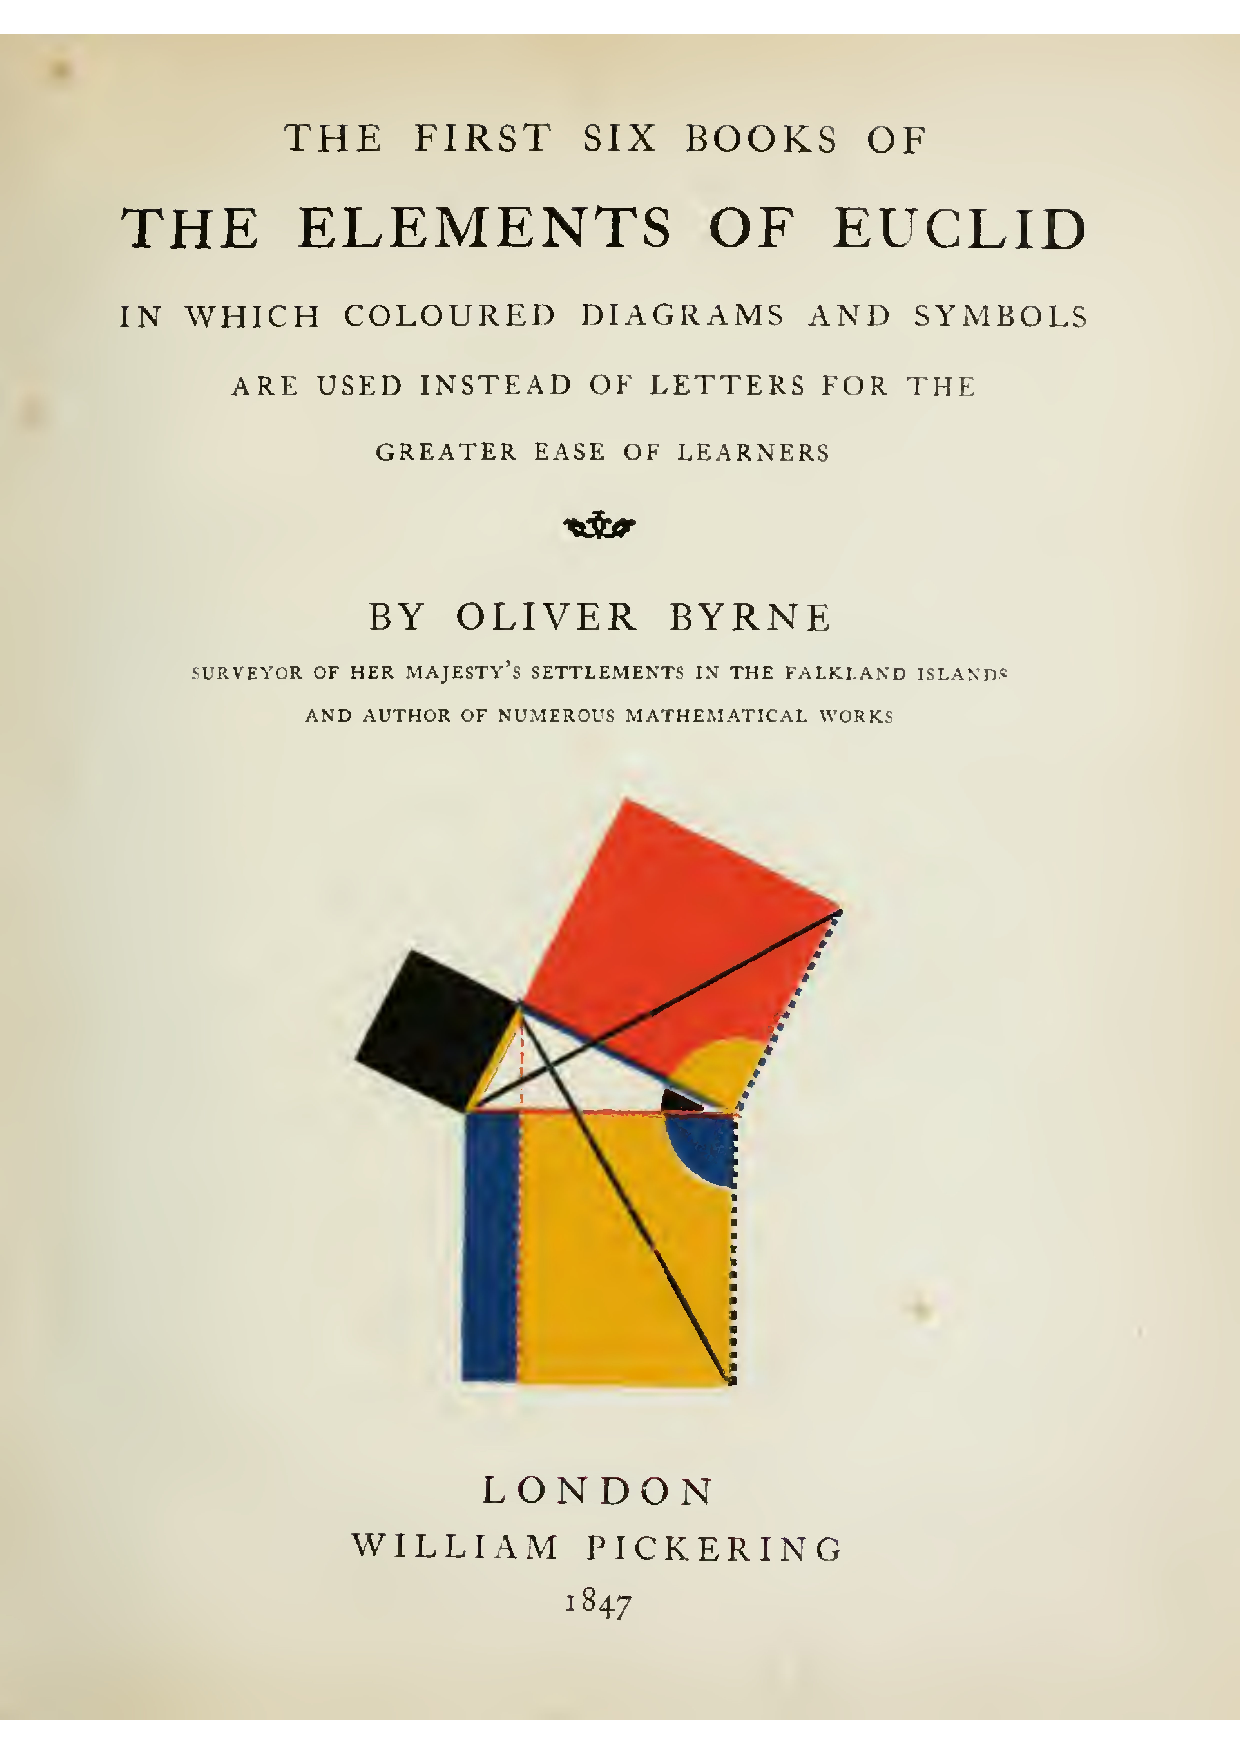
\includegraphics[height=\heighttt]{euclid5}\\
		Color edition, 1847
	\end{minipage}
	\begin{minipage}[b]{0.24\linewidth}
		\centering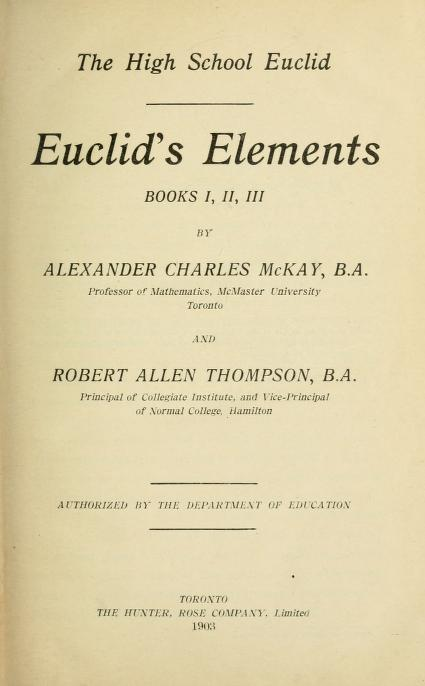
\includegraphics[height=\heighttt]{euclid4}\\
		Textbook, 1903
	\end{minipage}
\end{center}

Many of Euclid's arguments can be found \href{http://math.furman.edu/~jpoole/euclidselements/euclid.htm}{online}, and you can read Byrne's 1847 edition \href{http://math.uci.edu/~ndonalds/Elements-I-VI.pdf}{here}: the cover is Euclid's proof of the Pythagorean Theorem. We present an overview of Book I.

%to address some of the shortcomings in Euclid's original approach, it contains a more comprehensive list of definitions, has more axioms, and relabels propositions 4 and 5 as axioms (pages xviii--xxiii). 

\begin{description}\itemsep0pt
	\item[\normalfont\emph{Undefined Terms}] E.g., point, line, etc.\footnote{In fact Euclid attempted to define these: `A point is that which has no part,' and `A line has length but no breadth.'}
	\item[\normalfont\emph{Axioms/Postulates}]\negthickspace\!\footnote{%
		In Euclid, an axiom is somewhat more general than a postulate. Here the postulates contain the \emph{geometry.}%
	}\lstsp A1\lstsp If two objects equal a third, then the objects are equal\hfill ($=$ is transitive)\vspace{-5pt}
	\begin{itemize}
		\item[A2] If equals are added to equals, the results are equal\hfill ($a=c$ \& $b=d\implies a+b=c+d$)
		\item[A3] If equals are subtracted from equals, the results are equal
		\item[A4] Things that coincide are equal (in magnitude)
		\item[A5] The whole is greater than the part
		\item[P1] A pair of points may be joined to create a line
		\item[P2] A line may be extended
		\item[P3] Given a center and a radius, a circle may be drawn
		\item[P4] All right-angles are equal
		\item[P5] If a straight line crosses two others and the angles on one side sum to less than two right-angles then the two lines (when extended) meet on that side.
	\end{itemize}
\end{description}

\goodbreak

The first three postulates describe \emph{ruler and compass constructions.} P4 allows Euclid to compare angles at different locations. P5 is usually called the \emph{parallel postulate.}
\medbreak

Euclid's system doesn't quite fit the modern standard. Some axioms are vague (what are `things'?) and we'll consider several more-serious shortcomings later. For now we clarify two issues and introduce some notation.
\begin{description}
	\item[\normalfont\emph{Segments}] To Euclid, a line had \emph{finite} extent---we call such a \emph{(line) segment.} The segment joining points $A,B$ is denoted $\cl{AB}$. In modern geometry, a \emph{line} extends as far as permitted, often infinitely.
	\item[\normalfont\emph{Congruence}] Euclid uses \emph{equal} where modern mathematicians say \emph{congruent}. We'll express congruent segments and angles in the modern fashion, e.g., $\angle ABC\cong\angle DEF$. Equal angles/segments must be genuinely the same object (same location, etc.).
\end{description}


\boldsubsubsection{Basic Theorems à la Euclid}

Theorems were typically presented as a \emph{problem}. Euclid provides a constructive solution (P1--P3) before proving that his construction really does solve the problem.

\begin{thm}{I.\,1}{euclid1-1}
	Problem: to construct an equilateral triangle on a given segment.
\end{thm}

The labelling I.\,1 indicates Book I, Theorem 1. A triangle is equilateral if its three sides are congruent.

\begin{tcolorbox}[proofstyle, lower separated=false, sidebyside, sidebyside align=top seam, sidebyside gap=0pt, righthand width=0.35\linewidth]
	\emph{Proof.}\ \ Given a line segment $\cl{AB}$:\smallbreak
	By P3, construct circles centered at $A$ and $B$ with radius $\cl{AB}$.\smallbreak
	Call one of the intersection points $C$. By P1, construct $\cl{AC}$ and $\cl{BC}$.\smallbreak
	We claim that $\triangle ABC$ is equilateral.\medbreak
	Observe that $\cl{AB}$ and $\cl{AC}$ are radii of the circle centered at $A$, while $\cl{AB}$ and $\cl{BC}$ are radii of the circle centered at $B$. By Axiom A1, the three sides of $\triangle ABC$ are congruent.
	\tcblower
	\flushright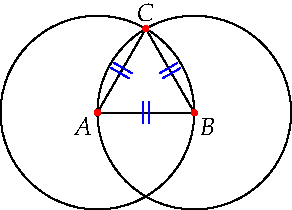
\includegraphics{euclid-I1}\hfil\qedsymbol
\end{tcolorbox}


Euclid proceeds to develop several well-known constructions and properties of triangles.
\begin{itemize}\itemsep0pt
  \item (I.\,4)\lstsp Side-angle-side (SAS) congruence: if two triangles have two pairs of congruent sides and the angles between these are congruent, then the remaining sides and angles are also congruent in pairs.
  \[
  	\begin{cases}
		  \cl{AB}\cong\cl{DE}\\
		  \angle ABC\cong\angle DEF\\
		  \cl{BC}\cong\cl{EF}
 	 	\end{cases}
  	\quad\implies
  	\begin{cases}
		  \cl{AC}\cong\cl{DF}\\
		  \angle BCA\cong\angle EFD\\
		  \angle CAB\cong\angle FDE
  	\end{cases}
  \]
  \item (I.\,5)\lstsp An isosceles triangle has congruent base angles.
  \item (I.\,9)\lstsp To bisect an angle.
  \item (I.\,10)\lstsp To find the midpoint of a segment.
  \item (I.\,15)\lstsp If two lines/segments cut one another, opposite angles are congruent.
\end{itemize}
Have a look at some of Euclid's arguments, say in Byrne's edition. These are worth reading despite the logical issues in Euclid's presentation. We'll revisit these basic results in the Exercises and in the next two sections. 

\goodbreak


\boldsubsubsection{Parallel Lines: Construction \& Existence}\phantomsection\label{pg:parallelexist}

\begin{defn}{}{parallel}
	Lines are \emph{parallel} if they do not intersect. Segments are parallel if no extensions of them intersect.
\end{defn}

In Euclid, a line is not parallel to itself. The next result is one of the most important in Euclidean geometry, for it describes how to create a parallel line through a given point.


\begin{thm}[lower separated=false, sidebyside, sidebyside align=top seam, sidebyside gap=0pt, righthand width=0.37\linewidth]{I.\,16\ Exterior Angle Theorem}{extangle}
	If one side of a triangle is extended, then the exterior angle is larger than either of the opposite interior angles.\smallbreak
	In the picture, we have $\delta>\alpha$ and $\delta>\beta$.
	\tcblower
	\flushright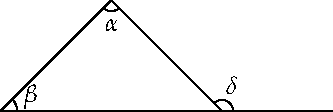
\includegraphics{euclid-I16}
\end{thm}

Euclid did not quantify angles numerically: $\delta>\alpha$ means that $\alpha$ is congruent to some angle \emph{inside} $\delta$.

\begin{proof}
	Construct the bisector $\cl{BM}$ of $\cl{AC}$ \ (I.\,10).\par
	\begin{minipage}[t]{0.64\linewidth}\vspace{-5pt}
		Extend $\cl{BM}$ to $E$ such that $\cl{BM}\cong\cl{ME}$ \  (I.\,2) and connect $\cl{CE}$ \  (P1).\smallbreak
		The opposite angles at $M$ are congruent \ (I.\,15).\smallbreak
		SAS (I.\,4) applied to $\triangle AMB$ and $\triangle CME$ says $\angle BAM\cong\angle EMC$, which is clearly smaller than the exterior angle at $C$.
	\end{minipage}
	\hfill
	\begin{minipage}[t]{0.35\linewidth}\vspace{-20pt}
		\flushright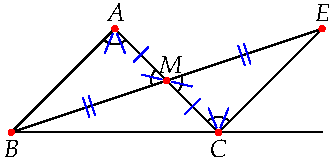
\includegraphics{euclid-I16p}
	\end{minipage}
	\smallbreak
	Bisect $\cl{BC}$ and repeat the argument to see that $\beta<\delta$.
\end{proof}

The proof in fact \emph{constructs} a parallel ($\cl{CE}$) to $\cl{AB}$ through $C$, as the next result shows.

\begin{thm}[lower separated=false, sidebyside, sidebyside align=top seam, sidebyside gap=0pt, righthand width=0.32\linewidth]{I.\,27}{}
	If a line falls on two other lines such that the alternate angles ($\alpha,\beta$) are congruent, then the two lines are parallel.
	\tcblower
	\flushright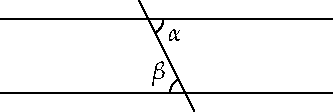
\includegraphics{euclid-I27}
\end{thm}

The \emph{alternate angles} in the exterior angle theorem are those at $A$ and $C$: $\cl{CE}$ really is parallel to $\cl{AB}$.

\begin{tcolorbox}[proofstyle,lower separated=false, sidebyside, sidebyside align=top seam, sidebyside gap=0pt, righthand width=0.37\linewidth]
	\emph{Proof.}\lstsp If the lines were not parallel, they would meet on one side. WLOG suppose they meet on the right side at $C$.\smallbreak
	The angle $\beta$ at $B$, being exterior to $\triangle ABC$, must be greater than the angle $\alpha$ at $A$ \ (I.\,16): contradiction.
	\tcblower
	\flushright
	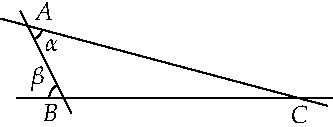
\includegraphics{euclid-I27p}\\[-12pt]\hfill\qedsymbol
\end{tcolorbox}

Euclid combines this with the vertical angles theorem (I.\,15) to finish the first half of Book I.

\begin{cor}[lower separated=false, sidebyside, sidebyside align=top seam, sidebyside gap=0pt, righthand width=0.32\linewidth]{I.\,28}{euclid28}
	If a line falling on two other lines makes congruent angles, then the two lines are parallel.
	\tcblower
	\flushright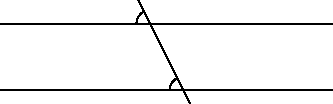
\includegraphics{euclid-I28}
\end{cor}


Thus far, Euclid uses only postulates P1--P4. In any model in which these hold:
\[
	\tcbhighmath{\text{Given a line $\ell$ and a point $C$ not on $\ell$, \textbf{there exists} a parallel to $\ell$ through $C$}}
\]
\goodbreak


\boldsubsubsection{Parallel Lines: Uniqueness, Angle-sums \& Playfair's Postulate}

Euclid finally invokes the parallel postulate to prove the converse of I.\,27, showing that the congruent alternate angle approach is the \emph{only} way to have parallel lines.

\begin{thm}{I.\,29}{euclid29}
	If a line falls on two parallel lines, then the alternate angles are congruent.
\end{thm}

\begin{tcolorbox}[proofstyle,lower separated=false, sidebyside, sidebyside align=top seam, sidebyside gap=0pt, righthand width=0.37\linewidth]
	\emph{Proof.}\ \ Given the picture, we must prove that $\alpha\cong\beta$.\smallbreak
	Suppose not and WLOG that $\alpha>\beta$.\smallbreak
	But then $\beta+\gamma<\alpha+\gamma$, which is a straight edge.\smallbreak
	By the parallel postulate, the lines $\ell,m$ meet on the left side of the picture, whence $\ell$ and $m$ are not parallel.
	\tcblower
	\flushright
	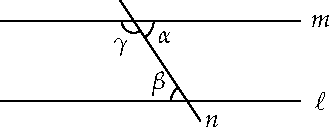
\includegraphics{euclid-I29}\\[-10pt]\qedsymbol
\end{tcolorbox}

The most well-known result about triangles is now within our grasp: the interior angles sum to a straight-edge. Euclid words this slightly differently.

\begin{thm}{I.\,32}{}
	If one side of a triangle is extended, the exterior angle is congruent to the sum of the opposite interior angles.
\end{thm}

\begin{minipage}[t]{0.64\linewidth}\vspace{-4pt}
	\emph{This is not a numerical sum,} though for the sake of familiarity we'll often write \ang{180} for a straight-edge and \ang{90} for a right-angle.\par
	In the picture we've labelled angles with Greek letters for clarity. The result amounts to showing that $\widetilde\alpha+\widetilde\beta\cong\alpha+\beta$.
\end{minipage}
\hfill
\begin{minipage}[t]{0.34\linewidth}\vspace{-9pt}
	\flushright
	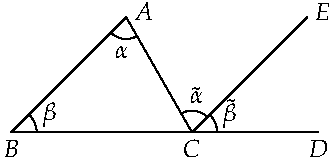
\includegraphics{euclid-I32}
\end{minipage}

\vspace{-20pt}

\begin{proof}
	Construct $\cl{CE}$ parallel to $\cl{BA}$ as in I.\,16, so that $\widetilde\alpha\cong\alpha$.\smallbreak
	$\cl{BD}$ falls on parallel lines $\cl{AB}$ and $\cl{CE}$, whence $\widetilde\beta\cong\beta$ (Corollary of I.\,29).\smallbreak
	Axiom A2 shows that $\angle ACD=\widetilde\alpha+\widetilde\beta\cong\alpha+\beta$.
\end{proof}


\medskip


The parallel postulate is stated in the negative (angles \emph{don't} sum to a straight-edge, therefore the lines are \emph{not} parallel). Euclid possibly chose this formulation to facilitate proofs by contradiction, though the unfortunate effect is to obscure the meaning of the parallel postulate. Here is a more modern interpretation.

\begin{axiom}[lower separated=false, sidebyside, sidebyside align=top seam, sidebyside gap=0pt, righthand width=0.37\linewidth]{Playfair's Postulate}{playfair}
	Given a line $\ell$ and a point $C$ not on $\ell$, \textbf{at most one} parallel $m$ to $\ell$ passes through $C$.
	\tcblower
	\flushright
	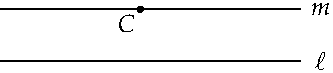
\includegraphics{euclid-playfair-defn}
\end{axiom}


\begin{minipage}[t]{0.62\linewidth}\vspace{0pt}
	Our discussion thus far shows that the parallel postulate implies Playfair.
	\begin{itemize}\itemsep0pt
	  \item Let $A,B\in\ell$ and construct the triangle $\triangle ABC$.
	  \item The exterior angle theorem constructs $E$ and thus a parallel $m$ to $\ell$ by I.\,27.
	  \item I.\,29 invokes the parallel postulate to prove that this is the \emph{only} such parallel.
	\end{itemize}
\end{minipage}
\hfill
\begin{minipage}[t]{0.37\linewidth}\vspace{0pt}
	\flushright
	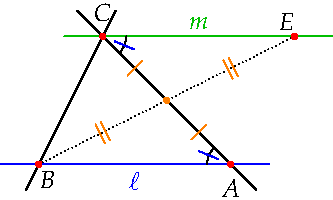
\includegraphics{euclid-playfair3}
\end{minipage}\bigbreak

In fact the postulates are equivalent.

\begin{thm}{}{}
	In the presence of Euclid's first four postulates, Playfair's postulate and the parallel postulate (P5) are equivalent.
\end{thm}

\begin{proof}
	\begin{description}
		\item[\normalfont (P5 $\Rightarrow$ Playfair)] We proved this above.
		\item[\normalfont (Playfair $\Rightarrow$ P5)] We prove the contrapositive. Assume postulates P1--P4 are true and that P5 is \emph{false.} Using quantifiers, and with reference to the picture in I.\,29, we restate the parallel postulate:
	\begin{quote}
	  P5:\lstsp $\forall$ pairs of lines $\ell,m$ and $\forall$ crossing lines $n$, \  $\beta+\gamma<\ang{180}\implies\ell,m$ \emph{not parallel.}
	\end{quote}
	\begin{minipage}[t]{0.62\linewidth}\vspace{-7pt}
		Its \emph{negation} (P5 false) is therefore:
		\begin{quote}
	  	$\exists$ parallel lines $\ell,m$ and a crossing line $n$ for which $\beta+\gamma<\ang{180}$
		\end{quote}
		This is without loss of generality: if $\beta+\gamma>\ang{180}$, consider the angles on the other side of $n$.\medbreak
		By the the exterior angle theorem/I.\,28, we may build a parallel line $\hat\ell$ to $\ell$ through the intersection $C$ of $m$ and $n$ (in the picture, $\hat\beta\cong\beta$). Crucially, this only requires postulates P1--P4!
	\end{minipage}
	\hfill
	\begin{minipage}[t]{0.37\linewidth}\vspace{0pt}
		\flushright
		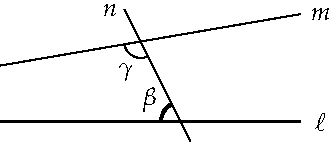
\includegraphics{euclid-playfair2}\\
		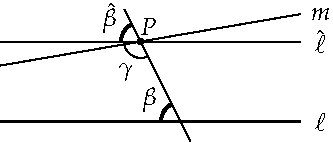
\includegraphics{euclid-playfair}
	\end{minipage}\smallbreak
	Observe that $\hat\ell$ and $m$ are \emph{distinct} since $\hat\beta+\gamma\cong\beta+\gamma<\ang{180}$.
	We therefore have a line $\ell$ and a point $C$ not on $\ell$, though which pass (at least) \emph{two} parallels to $\ell$: Playfair's postulate is \emph{false.} \qedhere
	\end{description}
\end{proof}



\boldsubsubsection{Non-Euclidean Geometry}\phantomsection\label{pg:sphere}

That Euclid waited so long before invoking the uniqueness of parallels suggests he was trying to establish as much as he could about triangles and basic geometry in its absence. By contrast, everything from I.\,29 onwards relies on the parallel postulate, including the proof that the angle sum in a triangle is \ang{180}. For centuries, many mathematicians believed, though none could prove it, that such a fundamental fact about triangles must be true independent of the parallel postulate.\smallbreak
Loosely speaking, a \emph{non-Euclidean geometry} is a model for which a parallel through an off-line point either doesn't exist or is non-unique. It wasn't until the 17--1800s and the development of \emph{hyperbolic geometry} (Chapter \ref{chap:hyper}) that a model was found in which Euclid's first four postulates hold but for which the parallel postulate is false.\footnote{This shows that the parallel postulate is independent; in fact all Euclid's postulates are independent. They are also consistent (the `usual' points and lines in the plane are a model), but incomplete: a sample undecidable is in Exercise \ref{ex:euclidundecideable}.}\par

\begin{minipage}[t]{0.76\linewidth}\vspace{-5pt}
	We shall eventually see that every triangle in hyperbolic geometry has angle sum less than \ang{180}, though this will require a lot of work! For a more easily visualized non-Euclidean geometry consider the sphere. A rubber band stretched between three points on its surface describes a \emph{spherical triangle}: an example with angle sum \ang{270} is drawn. A similar game can be played on a saddle-shaped surface: as in hyperbolic geometry, `triangles' will have angle sum less than \ang{180}.
\end{minipage}
\hfill
\begin{minipage}[t]{0.23\linewidth}\vspace{-10pt}
	\flushright
	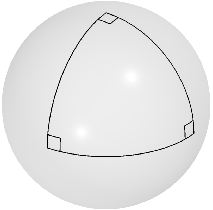
\includegraphics[scale=0.95]{euclid-sphere}
\end{minipage}

\goodbreak

\goodbreak


\boldsubsubsection{Pythagoras' Theorem}\phantomsection\label{pg:pythagoras}

Following his discussion of parallels, Euclid shows that parallelograms with the same base and height are equal (in area) (I.\,33--41), before providing constructions of parallelograms and squares (I.\,42--46). Some of this is in Exercise \ref{ex:pythagexs}. Immediately afterwards comes the capstone of Book I.


\begin{thm}{I.\,47 Pythagoras' Theorem}{}
	The square on the hypotenuse of a right triangle equals (has the same area as) the sum of the squares on the other sides.
\end{thm}

\begin{proof} 
	The given triangle $\triangle ABC$ is assumed to have a right-angle at $A$.\par
	\begin{minipage}[t]{0.6\linewidth}\vspace{0pt}
	\begin{enumerate}\itemsep0pt
	  \item Construct squares on each side of $\triangle ABC$ \ (I.\,46) and a parallel $\cl{AL}$ to $\cl{BD}$ \ (I.\,16).
	  \item $\cl{AB}\cong\cl{FB}$ and $\cl{BD}\cong\cl{BC}$ since sides of squares are congruent. Moreover $\angle ABD\cong\angle FBC$ since both contain \textcolor{blue}{$\angle ABC$} and a \textcolor{red}{right-angle}.
	  \item Side-angle-side (I.\,4) says that $\triangle ABD$ and $\triangle FBC$ are congruent (identical up to rotation by \ang{90}).
		\item I.\,41 compares areas of parallelograms and triangles with the same base and height:\vspace{0pt}
		\begin{align*}
			\operatorname{Area}(\textcolor{red}{\square ABFG})&=2\operatorname{Area}(\triangle FBC)\\
			&=2\operatorname{Area}(\triangle ABD)\\
			&=\operatorname{Area}\left(\textcolor{red}{\fbox{\phantom{'}}BOLD}\right)\\[-25pt]
		\end{align*}
		\item Similarly $\operatorname{Area}(\textcolor{Green}{\square ACKH}) =\operatorname{Area}\left(\textcolor{Green}{\fbox{\phantom{'}}OCEL}\right)$.
	\end{enumerate}
	\end{minipage}
	\hfill
	\begin{minipage}[t]{0.39\linewidth}\vspace{0pt}
		\flushright
		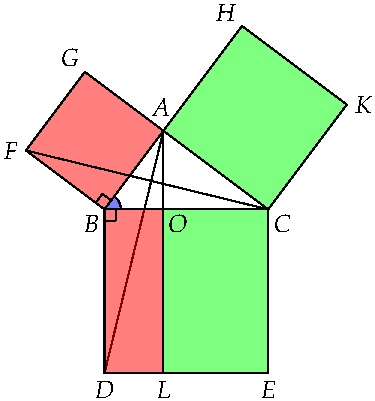
\includegraphics{euclid-I47}
	\end{minipage}
	\begin{enumerate}\setcounter{enumi}{5}
		\item Sum the rectangles to obtain $\square BCED$ and complete the proof.\hfill\qedhere
	\end{enumerate}
\end{proof}



Euclid finishes Book I with the converse, which we state without proof. Euclid's argument is very sneaky---look it up!

\begin{thm}{I.\,48}{}
	If the (areas of the) squares on two sides of a triangle equal the (area of the) square on the third side, then the  triangle has a right-angle opposite the third side.
\end{thm}

The \emph{Elements} contains thirteen books. Much of the remaining twelve discuss further geometric constructions, including in three dimensions. There is also a healthy dose of basic number theory including what is now known as the Euclidean algorithm.\medbreak

While undoubtedly a masterpiece of logical reasoning, Euclid's presentation has several flaws. Most problematic is his reliance on pictorial reasoning: for instance, he `proves' the SAS and SSS congruence theorems (I.\,4 \& 8) by laying one triangle on top of another, a process not justified by his axioms (look it up \href{http://math.furman.edu/~jpoole/euclidselements/euclid.htm}{online} or \href{http://math.uci.edu/~ndonalds/Elements-I-VI.pdf}{Byrne}). In a modern sense, Euclid's approach is part axiomatic system and part model: his reasoning requires a visual/physical representation of lines, circles, etc. Because of these issues, we now turn to a more modern description of Euclidean geometry, courtesy of David Hilbert.

\clearpage

% 
% \paragraph{Book II: Geometric algebra}
% 
% We tend to think of Pythagoras' Theorem as a statement in Geometric Algebra: i.e., $c^2=a^2+b^2$, but this is not how Euclid saw it. To Euclid, Geometric Algebra was about solving equations to find unknowns. Of course the concept of algebra hadn't been invented yet, so the very problems had to be stated geometrically. Such concerns comprise the bulk of Book II of the \emph{Elements,} and are mostly attributable to the Pythagoreans.Here is an example.
% 
% \begin{thm*}[II.\,11]
% A straight line can be divided so that the rectangle contained by the whole and one of the segments is equal to the square on the remaining segment.
% \end{thm*}
% 
% 
%  In our modern language we would say: given $AB=a$, find $H$ on $AB$, so that $AH=x$, with $x^2=a(a-x)$. Here is Euclid's proof.
% 
% \begin{minipage}{0.3\textwidth}
% 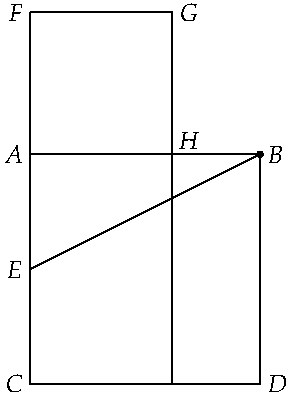
\includegraphics{geo-17-bk2}
% \end{minipage}\hfill
% \begin{minipage}{0.6\textwidth}
% \begin{enumerate}
%   \item Construct square $ABDC$ on $AB$
% 	\item Bisect $AC$; call midpoint $E$
% 	\item Connect $EB$
% 	\item Extend $AC$
% 	\item Lay off $EF=EB$ on $AC$ extended
% 	\item Construct square $FGHA$
% \end{enumerate}
% \end{minipage}
% 
%  In our modern language, with our understanding of Pythagoras', we see that Euclid has constructed $H$ so that $x=\frac{\sqrt 5-1}2a$. We can easily check that this solves the equation $x^2=a(a-x)$. Note that this is a construction of the golden ratio:
% \[AH:HB=1:\frac{\sqrt 5-1}2=\frac{\sqrt 5+1}2:1.\]
% For many centuries after Euclid, the meaning of `solve' was exactly this: construct a solution.


\begin{exercises}
	\hangindent\doubleind
	1. \ (a) \ Prove the \emph{vertical angle theorem} (I.\,15): if two lines cut one another, opposite angles are congruent.\vspace{-8pt}

	\begin{enumerate}\setcounter{enumi}{1}
	  \item[]\begin{enumerate}\setcounter{enumii}{1}
	    \item[](\emph{Hint: This is one place where you will need to use postulate 4 regarding right-angles})
	    \item Use part (a) to complete the proof of the exterior angle theorem: i.e.,\ explain why $\beta<\delta$.
	  \end{enumerate}
	
		\item\label{ex:pythagexs} To help prove Pythagoras', Euclid makes use of the following results. Prove them as best as you can. Full rigor is tricky, but the pictures should help!
		\begin{enumerate}
		  \item (I.\,11) At a given point on a line, to construct a perpendicular.
		  \item (I.\,46) To construct a square on a given segment.
		  \item (I.\,35) Parallelograms on the same base and with the same height have equal area.
		  \item (I.\,41) A parallelogram has twice the area of a triangle on the same base and with the same height.
		\end{enumerate}
		
		\begin{center}
			\begin{tabular}{c@{\quad}c@{\quad}c}
				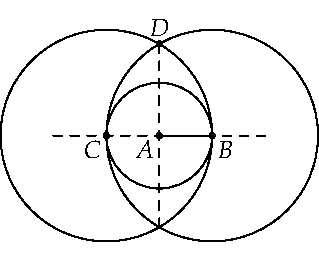
\includegraphics[scale=0.95]{euclid-I11}
				&
				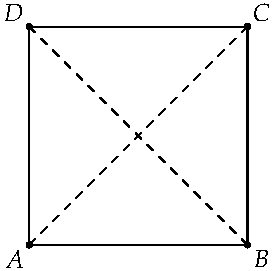
\includegraphics[scale=0.95]{euclid-I46}
				&
				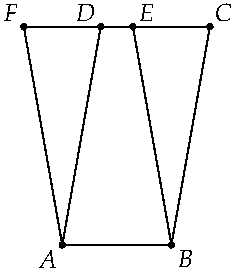
\includegraphics[scale=0.95]{euclid-I35a}
				\\[-2pt]
				Theorem I.\,11
				&
				Theorem I.\,46
				&
				Theorem I.\,35
			\end{tabular}
		\end{center}
		
	  
	  \item Consider spherical geometry (page \pageref{pg:sphere}), where \emph{lines} are paths of shortest distance (great circles).
	 	\begin{enumerate}
	 	  \item Which of Euclid's postulates P1--P5 are satisfied by this geometry?
	  	\item (Hard)\lstsp Where does the proof of the exterior angle theorem \emph{fail} in spherical geometry? 
	 	\end{enumerate}
	  
	  
	  \item\begin{enumerate}
	    \item State the negation of Playfair's postulate.
	    \item Prove that Playfair's postulate is equivalent to the following statement:
	 	 	\begin{quote}
	  		Whenever a line is perpendicular to one of two parallel lines, it must be perpendicular to the other.
	  	\end{quote}
	  \end{enumerate}
	 
	  
	  \item\label{ex:euclidundecideable} The \emph{line-circle continuity} property states:
	  \begin{quote}
	  	If point $P$ lies inside and $Q$ lies outside a circle $\alpha$, then the segment $\overline{PQ}$ intersects $\alpha$.
	  \end{quote}
	  By considering the set of rational points in the plane $\Q^2=\{(x,y):x,y\in\Q\}$, and making a sensible definition of line and circle, show that the line-circle continuity property is undecidable within Euclid's system.
		
		
		\item The standard proof of the converse of Pythagoras' theorem (I.\,48) is, in fact, a \emph{corollary} of the original! Look it up and explain the argument as best you can.
	\end{enumerate}
	
\end{exercises}

\clearpage



\subsection{Hilbert's Axioms I: Incidence and Order}\label{sec:hilbert1}

The long process of identifying and correcting the errors and omissions in Euclid's \emph{Elements} culminated in the 1899 publication of David Hilbert's \emph{Grundlagen der Geometrie (Foundations of Geometry)}. In the next two sections we consider some of the details of Hilbert's approach, providing a modern and logically superior description of Euclidean geometry.\smallbreak

Hilbert's axioms for plane geometry\footnote{%
	Like Euclid, Hilbert also covered 3D geometry---we only give the axioms sufficient for plane geometry. With regard to our desired properties (Definition \ref{defn:consistency}), his system is about as good as can be hoped: essentially one only one model exists, which is almost the same thing as completeness. In the absence of the continuity axiom, the axioms are consistent; in line with Gödel's theorems (\ref{thm:godel}), consistency cannot be proved once continuity is included. As stated, the axioms are not quite independent, though this can be remedied: O-3 does not require existence (follows from Pasch's axiom), C-1 does not require uniqueness (follows from uniqueness in C-4) and C-6 can be weakened slightly.%
} are listed on the next page. The undefined terms consist of two types of object (\emph{points} and \emph{lines}), and three relations (\emph{between $*$, on $\in$} and \emph{congruence $\cong$}). For brevity we'll often use/abuse set notation, viewing a line as a set of points, though this is not necessary. At various places, definitions and notations are required.

\begin{defn}{}{hilbertbasic}
	Throughout, $A,B,C$ denote points and $\ell,m$ lines.
	\begin{description}\itemsep 0pt plus 1pt
	  \item[\normalfont\emph{Line}:] $\smash[t]{\lin{AB}}$ denotes the line through distinct $A,B$. This exists and is unique by axioms I-1 and I-2.
	  \item[\normalfont\emph{Segment}:] $\cl{AB}:=\{A,B\}\cup\{C:A*C*B\}$ consists of distinct \emph{endpoints} $A,B$ and all \emph{interior} points $C$ lying between them.
	  \item[\normalfont\emph{Ray}:] $\ray{AB}:=\cl{AB}\cup\{C:A*B*C\}$ is a ray with \emph{vertex} $A$. In essence we extend $\cl{AB}$ beyond $B$.
	  \item[\normalfont\emph{Triangle}:] $\triangle ABC:=\cl{AB}\cup\cl{BC}\cup\cl{CA}$ where $A,B,C$ are non-collinear. Triangles are \emph{congruent} if their sides and angles are congruent in pairs.
		\item[\normalfont\emph{Sidedness}:] Distinct $A,B$, not on $\ell$, lie on the \emph{same side} of $\ell$ if $\cl{AB}\cap\ell=\emptyset$. Otherwise $A$ and $B$ lie on \emph{opposite sides} of $\ell$.
		\item[\normalfont\emph{Angle}:] $\angle BAC:=\ray{AB}\cup\ray{AC}$ has \emph{vertex} $A$ and \emph{sides} $\ray{AB}$ and $\ray{AC}$.
		\item[\normalfont\emph{Parallelism}:] Lines $\ell$ and $m$ \emph{intersect} if there exists a point lying on both: $\exists A\in\ell\cap m$. Lines are \emph{parallel} if they do not intersect. Segments/rays are parallel when the corresponding lines are parallel.
	\end{description}
	The pictures represent these notions in the usual model of Cartesian geometry.
	\begin{center}
		\begin{tabular}{@{}c@{\qquad}c@{\qquad}c@{\qquad}c@{}}
			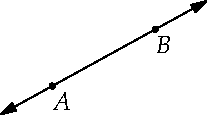
\includegraphics{hilbert-def-line}
			&
			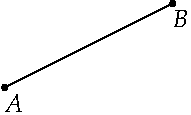
\includegraphics{hilbert-def-seg}
			&
			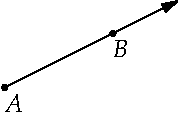
\includegraphics{hilbert-def-ray}
			&
			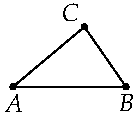
\includegraphics{hilbert-def-triangle}
			\\
			Line $\lin{AB}$
			&
			Segment $\cl{AB}$
			&
			Ray $\ray{AB}$
			&
			Triangle $\triangle ABC$
			\\[12pt]
			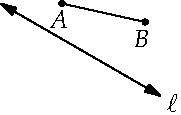
\includegraphics{hilbert-def-side}
			&
			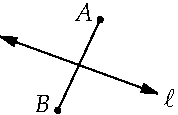
\includegraphics{hilbert-def-side2}
			&
			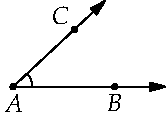
\includegraphics{hilbert-def-angle}
			&
			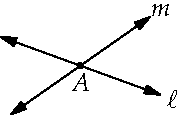
\includegraphics{hilbert-def-intersect}
			\\
			Same side
			&
			Opposite sides
			&
			Angle $\angle BAC$
			&
			Intersection $A\in\ell\cap m$
		\end{tabular}
	\end{center}
\end{defn}


\pagebreak
\thispagestyle{empty}
\begin{center}
\bfseries\Large Hilbert's Axioms for Plane Geometry
\end{center}

\begin{minipage}[t]{0.46\linewidth}
\boldinline{Undefined terms}
\begin{enumerate}\itemsep2pt
  \item \emph{Points}: \ use capital letters, $A,B,C\ldots$
  \item \emph{Lines}: \ use lower case letters, $\ell,m,n,\ldots$
  \item \emph{On}: \ $A\in\ell$ is read `$A$ lies on $\ell$'
  \item \emph{Between}: \ $A*B*C$ is read `$B$ lies between $A$ and $C$'
  \item \emph{Congruence}: \ $\cong$ is a binary relation on segments or angles
\end{enumerate}

\boldinline{Axioms of Incidence}

\begin{enumerate}
	\item[I-1] For any distinct $A,B$ there exists a line $\ell$ on which lie $A,B$.
	\item[I-2] There is at most one line through distinct $A,B$ \ ($A$ and $B$ both \emph{on} the line).
\end{enumerate}\vspace{-2pt}
	
Notation: \emph{line} $\overleftrightarrow{AB}$ through $A$ and $B$\vspace{-2pt}

\begin{enumerate}\setcounter{enumi}{2}	
	\item[I-3] On every line there exist at least two distinct points. There exist at least three points not all on the same line.
\end{enumerate}


\boldinline{Axioms of Order}

\begin{enumerate}
	\item[O-1] If $A*B*C$, then $A,B,C$ are distinct points on the same line and $C*B*A$.
	\item[O-2] Given distinct $A,B$, there is at least one point $C$ such that $A*B*C$.
	\item[O-3] If $A,B,C$ are distinct points on the same line, exactly one lies between the others.
\end{enumerate}\vspace{-2pt}
	
Definitions: \emph{segment} $\cl{AB}$ and \emph{triangle} $\triangle ABC$\vspace{-2pt}

\begin{enumerate}\setcounter{enumi}{3}	
	\item[O-4] (Pasch's Axiom) Let $\triangle ABC$ be a triangle and $\ell$ a line not containing any of $A,B,C$. If $\ell$ contains a point of the segment $\cl{AB}$, then it also contains a point of either $\cl{AC}$ or $\cl{BC}$. 
\end{enumerate}

Definitions: \emph{sides} of line $\overleftrightarrow{AB}$ and \emph{ray} $\ray{AB}$
\end{minipage}
\hfill
\begin{minipage}[t]{0.48\linewidth}
\boldinline{Axioms of Congruence}

\begin{enumerate}
  \item[C-1] (Segment transference) \ Let $A,B$ be distinct and $r$ a ray based at $A'$. Then there exists a unique point $B'\in r$ for which $\cl{AB}\cong\cl{A'B'}$. Moreover $\cl{AB}\cong\cl{BA}$.
  \item[C-2] If $\cl{AB}\cong\cl{EF}$ and $\cl{CD}\cong\cl{EF}$, then $\cl{AB}\cong\cl{CD}$.
  \item[C-3] If $A*B*C$, \ $A'*B'*C'$, \ $\cl{AB}\cong\cl{A'B'}$ and $\cl{BC}\cong\cl{B'C'}$, then $\cl{AC}\cong\cl{A'C'}$.
  \end{enumerate}
	
Definitions: \emph{angle} $\angle ABC$\vspace{-2pt}

\begin{enumerate}\setcounter{enumi}{3}
  \item[C-4] (Angle transference) \ Given $\angle BAC$ and $\ray{A'B'}$, there exists a unique ray $\ray{A'C'}$ on a given side of $\overleftrightarrow{A'B'}$ for which $\angle BAC\cong\angle B'A'C'$.
  \item[C-5] If $\angle ABC\cong\angle GHI$ and $\angle DEF\cong\angle GHI$, then $\angle ABC\cong\angle DEF$. Moreover, $\angle ABC\cong\angle CBA$.
  \item[C-6] (Side-angle-side) Given triangles $\triangle ABC$ and $\triangle A'B'C'$, if $\cl{AB}\cong\cl{A'B'}$, $\cl{AC}\cong\cl{A'C'}$, and $\angle BAC\cong\angle B'A'C'$, then the triangles are congruent.\footnotemark{}
\end{enumerate}

\boldinline{Axiom of Continuity}\phantom{bob}\smallbreak

Suppose $\ell$ is partitioned into non-empty subsets $\Sigma_1,\Sigma_2$ such that no point of $\Sigma_1$ lies between two points of $\Sigma_2$ and vice versa.\par
Then there exists a unique point $\mathcal O\in\ell$ satisfying $P_1*\mathcal O*P_2$, if and only if $\mathcal O\neq P_1$, $\mathcal O\neq P_2$ and one of $P_1$ or $P_2$ lies in $\Sigma_1$ and the other in $\Sigma_2$.\medbreak



\boldinline{Playfair's Axiom}\phantom{bob}\smallbreak

Definition: \emph{parallel lines}\smallbreak

Given a line $\ell$ and a point $P$ not on $\ell$, there exists at most one line through $P$ parallel to $\ell$.
\end{minipage}

\footnotetext{Its sides/angles are congruent in pairs. We extend congruence to other geometric objects similarly.}

\clearpage





\boldsubsubsection{Axioms of Incidence: Finite Geometries}

The axioms of incidence describe the relation \emph{on.} An \emph{incidence geometry} is any model satisfying axioms I-1, I-2, I-3. Perhaps surprisingly, there exist incidence geometries with \emph{finitely many points}!

\begin{examples}{}{fano}
	By I-3, an incidence geometry requires \emph{at least three} points.\par
	\begin{minipage}[t]{0.62\linewidth}\vspace{-5pt}
		A 3-point geometry exists, and is unique up to relabelling:\smallbreak
		I-3 says the points $A,B,C$ must be non-collinear. By I-1 and I-2, each pair lies on a unique line, whence there are precisely three lines
		\[
			\ell=\{A,B\},\quad m=\{A,C\},\quad n=\{B,C\}
		\]
		Up to relabelling, there are two incidence geometries with four points: one is drawn; how many lines has the other?
	\end{minipage}
	\hfill
	\begin{minipage}[t]{0.37\linewidth}\vspace{-15pt}
		\flushright
		\begin{tabular}{cc@{}}
			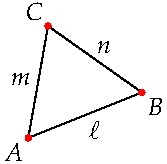
\includegraphics{hilbert-incidence3}
			&
			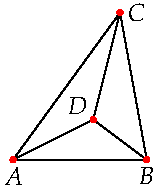
\includegraphics{hilbert-incidence4}\\
			3 points, 3 lines
			&
			%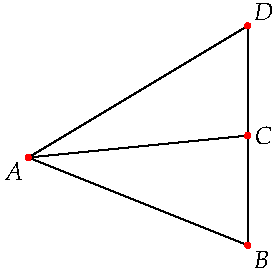
\includegraphics{hilbert-incidence4-2}
			4 points, 6 lines%&4 points, 4 lines
		\end{tabular}
	\end{minipage}
	\smallbreak
	\begin{minipage}[t]{0.72\linewidth}\vspace{0pt}
		The final picture is a seven-point incidence geometry called the \emph{Fano plane,} which finds many applications particularly in combinatorics. Each point lies on precisely three lines and each line contains precisely three points---each dot is colored to indicate the lines to which it belongs. Don't be fooled by the black line looking `curved' and seeming to cross the blue line near the top, for the line only contains three points!
	\end{minipage}
	\hfill
	\begin{minipage}[t]{0.27\linewidth}\vspace{-17pt}
		\flushright
		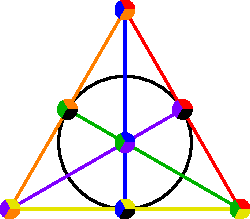
\includegraphics{hilbert-incidence7}
	\end{minipage}
\end{examples}

We can even prove some simple theorems in incidence geometry. The second is an exercise.

\begin{lemm}{}{intersectunique}
	If distinct lines intersect, then they do so in exactly one point.
\end{lemm}

\begin{proof}
	Suppose $A,B$ are distinct points of intersection. By axiom I-2, there is at most one line through $A$ and $B$. Contradiction.
\end{proof}

\begin{lemm}{}{incidenceeasy}
	Given any point, there exist at least two lines on which it lies.
\end{lemm}

%While incidence geometry is fun, our main goal is to understand Euclidean geometry, so we move on to the next set of axioms.





\begin{minipage}[t]{0.79\linewidth}\vspace{0pt}

\boldsubsubsection{Axioms of Order: Sides of a Line, Pasch's Axiom \& the Crossbar Theorem}

The order axioms describe the ternary relation \emph{between.} The first three make explicit the idea that points on a line lie in a fixed order: travelling along a line, one encounters each point exactly once. In particular, these axioms prevent `circular' lines (the pictured contradiction), and guarantee that a line contains infinitely many points.\smallbreak
Each of the above finite incidence examples fails to satisfy (some of) the order axioms.
\end{minipage}
\hfill
\begin{minipage}[t]{0.2\linewidth}\vspace{0pt}
	\flushright
	\begin{tabular}{@{}c@{}}
		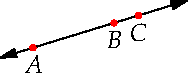
\includegraphics[scale=0.9]{hilbert-order}\\[-2pt]
		$A*B*C$ \checkmark\\[10pt]
		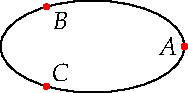
\includegraphics[scale=0.9]{hilbert-order2}\\
		Contradiction
	\end{tabular}
\end{minipage}\smallbreak

The rest of this section is devoted to the consequences of Pasch's axiom (O-4)---named to honor the work of Moritz Pasch (c.\,1882). Amongst other things, it permits us to define the \emph{interiors} of several geometric objects and to see that these are non-empty. For instance:

\begin{lemm}{Exercise \ref{exs:seginterior}}{seginterior}
	Every segment contains an interior point.
\end{lemm}

% We leave the proof to Exercise \ref{exs:seginterior}. By inducting on the Lemma, every segment contains \emph{infinitely many} points, whence the above finite geometries are not valid models once the order axioms are included.

\goodbreak

To get much further, it is necessary to establish that a line has precisely two \emph{sides} (Definition \ref{defn:hilbertbasic}). This concept lies behind several of Euclid's arguments, without being properly defined in the \emph{Elements.}


\begin{thm}{Plane Separation}{planesep}
	A line $\ell$ separates all points not on $\ell$ into two half-planes: the two \emph{sides} of $\ell$. To be explicit, suppose none of the points $A,B,C$ lie on $\ell$, then:
	\begin{enumerate}\itemsep0pt
	  \item If $A,B$ lie on the same side of $\ell$ and $B,C$ lie on the same side, then $A,C$ lie on the same side.
	  \item If $A,B$ lie on opposite sides and $B,C$ lie on opposite sides, then $A,C$ lie on the same side.
	  \item If $A,B$ lie on opposite sides and $B,C$ lie on the same side, then $A,C$ lie on opposite sides.
	\end{enumerate}\vspace{-10pt}
	\begin{center}
		\begin{tabular}{c@{\qquad}c@{\qquad}c}
			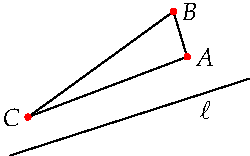
\includegraphics{hilbert-planesep}
			&
			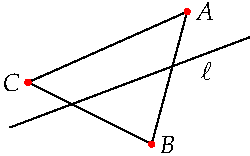
\includegraphics{hilbert-planesep2}
			&
			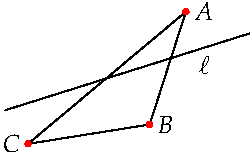
\includegraphics{hilbert-planesep3}
			\\
			Case 1
			&
			Case 2
			&
			Case 3
		\end{tabular}
	\end{center}
\end{thm}

\begin{proof}
	We prove the contrapositive of case 1. Suppose $A,B,C$ are non-collinear. If $\cl{AC}$ intersects $\ell$, then $\ell$ intersects one side of $\triangle ABC$. By Pasch's axiom, it also intersects either $\cl{AB}$ or $\cl{BC}$.\smallbreak
	The other cases are exercises, and we omit the tedious collinear possibilities.
\end{proof}

Plane separation/sidedness allows us to properly define interiors of angles and triangles. 

\begin{defn}{}{interiorangle}
	A point $I$ is \emph{interior} to angle $\angle BAC$ if:\par
	\begin{minipage}[t]{0.6\linewidth}\vspace{0pt}
		\begin{itemize}\itemsep0pt
	  	\item $I$ lies on the same side of $\lin{AB}$ as $C$, and,
	  	\item $I$ lies on the same side of $\lin{AC}$ as $B$.
		\end{itemize}
		Otherwise said, $I$ lies in the intersection of two half-planes.
	\end{minipage}
	\hfill
	\begin{minipage}[t]{0.35\linewidth}\vspace{-20pt}
		\flushright
		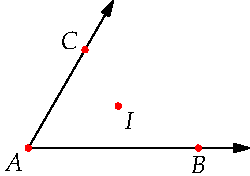
\includegraphics[scale=0.95]{hilbert-interior}
	\end{minipage}\medbreak
	
	A point $I$ is \emph{interior} to triangle $\triangle ABC$ if it is interior to all three of its angles $\angle ABC$, $\angle BAC$ and $\angle ACB$. Otherwise said, $I$ lies in the triple intersection of three of the half-planes defined by the triangle's sides.
\end{defn}

Interior points permit us to compare angles which share a vertex: if $I$ is interior to $\angle BAC$, then $\angle BAI<\angle BAC$ has obvious meaning \emph{without resorting to numerical angle measure.}

\begin{cor}{}{angleinteriorexist}
	Every angle has an interior point.
\end{cor}

\begin{proof}
	Given $\angle BAC$, consider any interior point $I$ of the segment $\cl{BC}$. This plainly lies on the same side of $\lin{AB}$ as $C$ and on the same side of $\lin{AC}$ as $B$.
\end{proof}

In Exercise \ref{exs:seginfinite}, we check that the interior of a triangle is non-empty.
\vfil

\goodbreak

Pasch's axiom could be paraphrased: \emph{If a line enters a triangle, it must come out.} We haven't quite established this crucial fact, however. What if the line passes through a vertex?

\goodbreak
 
\begin{thm}[lower separated=false, sidebyside, sidebyside align=top seam, sidebyside gap=0pt, righthand width=0.3\linewidth]{Crossbar Theorem}{}
	Suppose $I$ is interior to $\angle BAC$. Then $\ray{AI}$ intersects $\cl{BC}$.\medbreak
In particular, if a line passes through a vertex and an interior point of a triangle, then it intersects the side opposite the vertex.
	\tcblower
	\flushright
	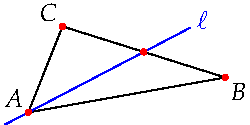
\includegraphics{hilbert-pasch2}
\end{thm}


\begin{proof}
	Extend $\cl{AB}$ to a point $D$ such that $A$ lies between $B$ and $D$ (O-2). Since $C$ is not on $\lin{BD}=\lin{AB}$ we have a triangle $\triangle BCD$. Since $\lin{AI}$ intersects one edge of $\triangle BCD$ at $A$ and does not cross any vertices (think about why\ldots), Pasch says it intersects one of the other edges ($\cl{BC}$ or $\cl{CD}$) at some point $M$.\smallbreak
	The result follows from applying plane separation to the lines $\lin{AB}=\lin{BD}$ and $\lin{AC}$. First observe:
	\begin{quote}
		Since $I,M$ lie on the same side of $\smash{\lin{AB}=\lin{BD}}$ as $C$, it follows that $\smash{\cl{IM}}$ does not intersect $\smash{\lin{AB}}$. Since $A,I,M$ are collinear and $A\in\lin{AB}$, it follows that \textcolor{red}{$A\notin\cl{IM}$}.
	\end{quote}
	If $M\in\cl{BC}$, we are done. Our goal is to show that $M\in\cl{CD}$ is a contradiction.\vspace{-5pt}
	\begin{center}
		\begin{tabular}{cc}
			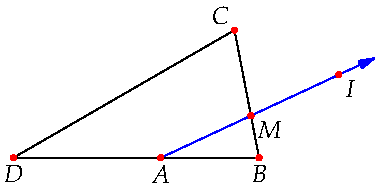
\includegraphics[scale=0.95]{hilbert-crossbar1}
			&
			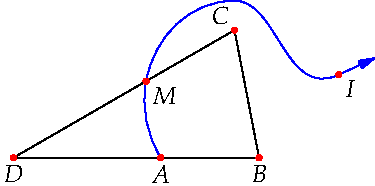
\includegraphics[scale=0.95]{hilbert-crossbar2}
			\\
			correct arrangement\footnotemark{}
			&
			contradiction
		\end{tabular}
	\end{center}
	Suppose, for contradiction, that $M\in\cl{CD}$. Relative to $\lin{AC}$:
	\begin{itemize}\itemsep0pt
		\item $I$ and $B$ lie on the same side since $I$ is interior to $\angle BAC$;
		\item $B$ and $D$ lie on opposite sides, since $B*A*D$ and $\lin{AC}\neq\lin{BD}=\cl{AB}$;
		\item $D$ and $M$ lie on the same side since $M\in\cl{CD}$ and $\lin{CD}\neq\lin{AC}$.		  
	\end{itemize}
	By plane separation, $I,M$ lie on opposite sides of $\lin{AC}$. The collinearity of $A,I,M$ then forces the contradiction \textcolor{red}{$A\in\cl{IM}$}.
\end{proof}

\footnotetext{The pictures could be modified: e.g., $I=M$ and $A*I*M$ are also correct arrangements ($M\in\cl{BC}$).}


\begin{minipage}[t]{0.67\linewidth}\vspace{-8pt}
	Euclid repeatedly uses the crossbar theorem without justification, including in his construction of perpendiculars and angle/segment bisectors (Theorems I.\,9+10). We sketch the latter here.\smallbreak
	Given $\angle BAC$, construct $E$ such that $\cl{AB}\cong\cl{AE}$. Construct $D$ using an equilateral triangle (I.\,1). SSS (I.\,8) shows that $\angle BAC$ is bisected, and SAS (I.\,4) that $\ray{AD}$ bisects $\cl{BE}$.\smallbreak
	Quite apart from Euclid's arguments for SAS and SSS being suspect (we'll deal with these in the next section), he gives no argument for why $D$ is interior to $\angle BAC$ or why $\ray{AD}$ should intersect $\cl{BE}$!
\end{minipage}
\hfill
\begin{minipage}[t]{0.32\linewidth}\vspace{0pt}
	\flushright
	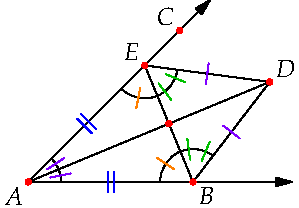
\includegraphics{hilbert-bisect}
\end{minipage}
\medbreak


Even with Pasch's axiom and the crossbar theorem, it requires some effort to repair Euclid's proof. No matter, we'll provide an alternative construction of the bisector once we've considered congruence.

\goodbreak


\begin{exercises}
	\exstart Label the vertices in the Fano plane 1 through 7 (any way you like). As we did in Example \ref{ex:fano} for the 3-point geometry, describe each line in terms of its points.
	\begin{enumerate}\setcounter{enumi}{1}
	  \item Prove Lemma \ref{lemm:incidenceeasy}.
	  
	  
	  \item\begin{enumerate}
	    \item Give a model for each of the 5-point incidence geometries. How many are there?\par
	  	(\emph{Hint: remember that order doesn't matter, so the only issue is how many points lie on each line})
	  	\item It is possible for there to be a 6-point incidence geometry so that each line contains precisely three points? Why/why not? 
	  \end{enumerate} 
	  
	    
	  \item Consider the proof of the crossbar theorem. How can we be certain that $\smash[t]{\lin{AI}}$ does not contain any of the vertices of $\triangle BCD$.
	  
	  
	  \item\label{exs:seginterior} You are given distinct points $A,B$. Using the axioms of incidence and order and Lemma \ref{lemm:intersectunique} (follows from I-2), show the existence of each of the points $C,D,E,F$ in the picture \emph{in alphabetical order.} Hence conclude the existence of a point $F$ lying \emph{between} $A$ and $B$ (Lemma \ref{lemm:seginterior}).\par
	  \begin{minipage}[t]{0.65\linewidth}\vspace{-5pt}
	  During your construction, address the following issues:
	  \begin{enumerate}\itemsep0pt
	    \item Explain why $D$ does not lie on $\overleftrightarrow{AB}$.
			\item Explain why $E$ does not lie on $\triangle ABD$.
			\item Explain why $E\neq C$ (whence $\overleftrightarrow{CE}$ exists).
			\item Explain why $F$ lies on $\cl{AB}$ and \emph{not} on $\cl{BD}$.
		\end{enumerate}
	  \end{minipage}
	  \hfill
	  \begin{minipage}[t]{0.34\linewidth}\vspace{-5pt}
	  	\flushright
	  	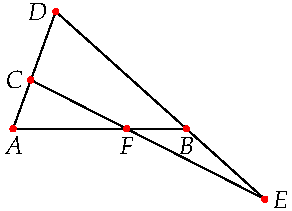
\includegraphics[scale=0.9]{hilbert-between}
	  \end{minipage}
	  
	  
	  \item\label{exs:bernays} We complete the proof of the plane separation theorem (\ref{thm:planesep}).
	  \begin{enumerate}
	    \item Prove part 3 (it is almost a verbatim application of Pasch's axiom).\par
	    \begin{minipage}[t]{0.75\linewidth}\vspace{-5pt}
	    \item Suppose a line $\ell$ intersects all three sides of $\triangle ABC$ but no vertices. This results in a very strange picture (we've labelled the intersections $D,E,F$ and WLOG chosen $D*E*F$).\smallbreak
	    Apply Pasch's axiom to $\triangle DBF$ and $\lin{AC}$ to obtain a contradiction. Hence establish part 2 of the plane separation theorem.    
	    \end{minipage}
	    \hfill
	    \begin{minipage}[t]{0.24\linewidth}\vspace{-35pt}
	    	\flushright
	    	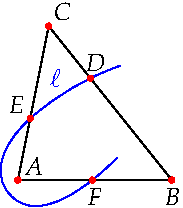
\includegraphics{hilbert-bernays}
	    \end{minipage}
	  \end{enumerate}
	  
	  
	  \item Suppose $A,B,C$ are distinct points on a line $\ell$.
	  \begin{enumerate}
	    \item Explain why there exists a line $m\neq \ell$ such that $B\in m$.
	    \item Prove that $A*B*C\iff A$ and $C$ lie on opposite sides of $m$.
	    \item Suppose $A*B*C$. Use part (b) to prove the following:
	    \begin{enumerate}
				\item $B$ is the only point common to the rays $\ray{BA}$ and $\ray{BC}$.
				\item If $D\in\ell$ is any point other than $B$, prove that $D$ lies in precisely one of $\ray{BA}$ or $\ray{BC}$.
			\end{enumerate}
	  \end{enumerate}
	  
	  
	  \item\label{exs:seginfinite} Prove that the interior of a triangle is non-empty.\par
	  (\emph{Hint: use Exercise \ref{exs:seginterior} to construct a suitable $I$, then prove that it lies on the correct side of each edge})
	  
	  
	  \item The existence of infinitely many points on a line follows easily from the fact that every segment has an interior point. Find an alternative proof that does not depend on Pasch's axiom.
	  
	\end{enumerate}
\end{exercises}


\clearpage



\subsection{Hilbert's Axioms II: Congruence}\label{sec:hilbert2}

Hilbert's congruence axioms address two primary issues in Euclid.
\begin{enumerate}
  \item Euclid's use of \emph{equal} is confusing. In Hilbert, segments/angles are now equal only when they are precisely the same (this amounts to the \emph{reflexivity} part of the next result).
  \item Euclid's frequent and unjustified use of pictorial reasoning. We previously discussed Euclid's erroneous approach to the SAS and SSS triangle congruence theorems. It was eventually realized that one of the triangle congruences has to be an axiom: SAS is Hilbert's C-6.
\end{enumerate}

We start with a small piece of bookkeeping.

\begin{lemm}{}{}
	Congruence of segments/angles is an equivalence relation.
\end{lemm}

\begin{proof}
	\begin{description}\itemsep0pt
  	\item[\normalfont(\emph{Reflexivity})] Let $\cl{AB}$ be given. Apply C-1 to obtain %\footnote{You could even take $A'=A$ and use the ray $r=\ray{AB}$!}
  	$\cl{A'B'}$ such that $\cl{AB}\cong\cl{A'B'}$. We sneakily use this \emph{twice} and apply C-2 to obtain
  	\[
  		\cl{AB}\cong\cl{A'B'}\text{ and } \cl{AB}\cong\cl{A'B'}\implies \cl{AB}\cong\cl{AB}
  	\]
  	\item[\normalfont(\emph{Symmetry})] Assume $\cl{AB}\cong\cl{CD}$. By reflexivity, $\cl{CD}\cong\cl{CD}$. By C-2 we have $\cl{CD}\cong\cl{AB}$.
  	\item[\normalfont(\emph{Transitivity})] Suppose $\cl{AB}\cong\cl{CD}$ and $\cl{CD}\cong\cl{EF}$. By symmetry, $\cl{EF}\cong\cl{CD}$. Axiom C-2 now shows that $\cl{AB}\cong\cl{EF}$.
  \end{description}
  \medskip
  Axioms C-4 and C-5 say essentially the same thing for angles (see Exercise \ref{exs:angcongequivrel}).
\end{proof}


\boldsubsubsection{Segment/Angle Transfer and Comparison}

Hilbert's axioms of segment and angle transference are crucial for comparing non-collinear segments and angles with distinct vertices.


\begin{defn}[lower separated=false, sidebyside, sidebyside align=top seam, sidebyside gap=0pt, righthand width=0.35\linewidth]{}{lengthcomp}
	Let segments $\cl{AB}$ and $\cl{CD}$ be given.\smallbreak
	By axiom C-1, let $E$ be the unique point on $\ray{CD}$ such that $\cl{CE}\cong\cl{AB}$: we have \emph{transferred} $\cl{AB}$ onto $\ray{CD}$.\smallbreak
	We write $\cl{AB}<\cl{CD}$ if $E$ lies between $C$ and $D$, etc.
	\tcblower
	\flushright
	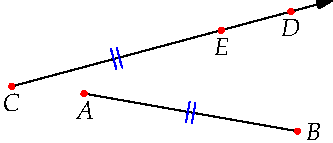
\includegraphics[scale=0.95]{angles-compare}
\end{defn}

By O-3, any two segments are comparable: given $\cl{AB}$ \& $\cl{CD}$, precisely one of the following holds,
\[
	\cl{AB}<\cl{CD}, \qquad \cl{CD}<\cl{AB}, \qquad\cl{AB}\cong\cl{CD}
\]
C-3 says that congruence respects the `addition' of adjacent congruent segments. Unique angle transfer, comparison and addition follow similarly from axiom C-4 and Definition \ref{defn:interiorangle} (interior points).\smallbreak

Neither Hilbert nor Euclid use or require an \emph{absolute} notion of length/angle-measure: the comparison $\cl{AB}<\cl{CD}$ does \emph{not} indicate a relationship between numerical quantities (lengths). Introducing numerical length requires the inclusion of the real numbers (and thus far more axioms)---for purity reasons, we postpone this until Section \ref{sec:similar}.
 

\goodbreak

\boldsubsubsection{The Triangle Congruence Theorems: SAS, ASA, SSS \& SAA}

Hilbert assumes side-angle-side (SAS) and proceeds to prove the remainder. Here is the first of these; we'll cover SSS momentarily and SAA in Exercise \ref{exs:saaproof}.

\begin{thm}{Angle-Side-Angle/ASA, Euclid I.\,26, case I}{asa}
	Suppose $\triangle ABC$ and $\triangle DEF$ satisfy
	\[
		\textcolor{Magenta}{\angle ABC}\cong\textcolor{Magenta}{\angle DEF},\qquad \textcolor{blue}{\cl{AB}}\cong\textcolor{blue}{\cl{DE}},\qquad \textcolor{red}{\angle BAC}\cong\textcolor{red}{\angle EDF}
	\]
	Then the triangles are congruent \ ($\angle ACB\cong\angle DFE$, \ $\cl{AC}\cong\cl{DF}$ and $\cl{BC}\cong\cl{EF}$).
\end{thm}

%We aren't (yet!) assuming uniqueness of parallels, so we cannot assert $\angle ACB\cong\angle DFE$.

Hilbert's approach modifies Euclid's: instead of laying $\triangle ABC$ on top of $\triangle DEF$, he creates a new triangle $\triangle DEG\cong \triangle ABC$ and proves that $G=F$.

\begin{proof}
	Segment transfer provides the unique point $G\in \ray{EF}$ such that $\textcolor{Green}{\cl{EG}}\cong \textcolor{Green}{\cl{BC}}$.\par
	\begin{minipage}[t]{0.65\linewidth}\vspace{0pt}
		SAS applied to $\textcolor{blue}{\cl{AB}}\cong\textcolor{blue}{\cl{DE}}$, $\textcolor{Magenta}{\angle ABC}\cong\textcolor{Magenta}{\angle DEG}\, (=\textcolor{Magenta}{\angle DEF})$, $\textcolor{Green}{\cl{BC}}\cong \textcolor{Green}{\cl{EG}}$, says $\textcolor{red}{\angle BAC}\cong \textcolor{red}{\angle EDG}\, (\cong \textcolor{red}{\angle EDF}$) (this last is by assumption).\smallbreak
		Since $F$ and $G$ lie on the same side of $\lin{DE}$, angle transfer (C-4) says they lie on the \emph{same ray} through $D$.\smallbreak
		But then $F$ and $G$ both lie on two distinct lines ($\lin{EF}=\lin{EG}$ and $\lin{DF}=\lin{DG}$). We conclude that $F=G$.\smallbreak
		By SAS we conclude that $\triangle ABC\cong\triangle DEF$.
	\end{minipage}
	\hfill
	\begin{minipage}[t]{0.34\linewidth}\vspace{-28pt}
		\flushright
		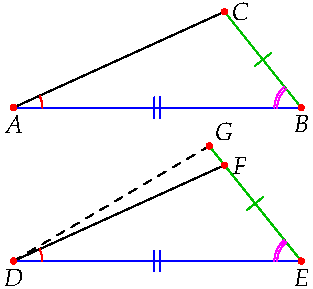
\includegraphics[scale=0.95]{angles-asa}
	\end{minipage}
\end{proof}




\boldsubsubsection{Geometry Without Circles}

Circles are at the heart of Euclid's constructions. Yet, for reason we'll address in Section \ref{sec:circ}, Hilbert essentially ignores them. We sketch a few of his alternative approaches to Euclid's basic results.

\begin{thm}{Euclid I.\,5}{euclidiso}
	An isosceles triangle has congruent base angles.
\end{thm}

Isosceles means \emph{equal legs}: two sides of the triangle are congruent. The remaining side is the \emph{base.} Euclid's argument relies on a famously complicated construction (look it up!). Hilbert does things more speedily and sneakily, by relabelling the original triangle and applying SAS.

\begin{tcolorbox}[proofstyle]
	\begin{minipage}[t]{0.7\linewidth}\vspace{0pt}
		\emph{Proof.}\lstsp Suppose $\triangle ABC$ is isosceles where $\textcolor{blue}{\cl{AB}}\cong\textcolor{blue}{\cl{AC}}$. Consider a `new' triangle $\triangle A'B'C'=\triangle ACB$ where the base points are switched:
		\[
			A':=A,\qquad B':=C,\qquad C':=B
		\]
		Observe:
		\begin{itemize}
		  \item $\textcolor{Green}{\angle BAC}\cong\textcolor{Green}{\angle CAB}$ (axiom C-5) $\implies\textcolor{Green}{\angle BAC}\cong\textcolor{Green}{\angle B'A'C'}$.
		  \item $\textcolor{blue}{\cl{AB}}\cong\textcolor{blue}{\cl{AC}}\implies \textcolor{blue}{\cl{AB}}\cong\textcolor{blue}{\cl{A'B'}}$ and $\textcolor{blue}{\cl{AC}}\cong\textcolor{blue}{\cl{A'C'}}$.
		\end{itemize}
		SAS says that $\angle ABC\cong\angle A'B'C'\cong\angle ACB$.
	\end{minipage}
	\hfill
	\begin{minipage}[t]{0.29\linewidth}\vspace{0pt}
		\flushright
		\includegraphics{angles-isos2}\\[-8pt]
		\hfill\qedsymbol
	\end{minipage}
\end{tcolorbox}


\goodbreak


\boldinline{Dropping a Perpendicular}

As with the majority of Book I, Euclid accomplishes this using circle intersections.\footnote{Consider the picture for Thm.\,I.\,11 in Exercise \ref*{sec:hilbert1}.\ref{ex:pythagexs}.} Hilbert instead uses segment/angle transference and the concept of sidedness.\par
	
\begin{minipage}[t]{0.69\linewidth}\vspace{0pt}
	Suppose we are given a line $\ell$ and a point $P$ not on $\ell$. Our goal is to construct a point $M\in\ell$ such that $\cl{PM}$ intersects $\ell$ in a right-angle.\smallbreak
	Let $A,B$ be distinct points on $\ell$ (axiom I-3) so that $\ell=\lin{AB}$.\smallbreak
	By axioms C-4 and C-1, we may transfer \textcolor{blue}{$\cl{AP}$} to the other side of $\ell$ at $A$, creating a new point $Q$.\smallbreak
	Since $P$ and $Q$ lie on opposite sides of $\ell$, the line intersects $\cl{PQ}$ at some point $M$. There are two cases to consider.
	\begin{itemize}
	  \item In the generic case $M\neq A$ (pictured), SAS applied to $\triangle MAP$ and $\triangle MAQ$ shows that $\angle AMP\cong\angle AMQ$. Since these angles sum to a straight edge ($\cl{PQ}$), they are both right-angles.
	  \item	In the extreme case $M=A$, there are no triangles and SAS cannot be applied. Instead, observe that $B$ does not lie on $\cl{PQ}$ (which axioms/results make this clear?!) and apply the above argument with $B$ instead of $A$.
	\end{itemize}
\end{minipage}
\hfill
\begin{minipage}[t]{0.29\linewidth}\vspace{0pt}
	\flushright
	\includegraphics[scale=1]{angles-perp}
\end{minipage}
\bigbreak

A generalization of this construction facilitates a corrected argument for the SSS triangle congruence.

\begin{thm}{Side-Side-Side/SSS, Euclid I.\,8}{}
	Suppose $\triangle ABC$ and $\triangle DEF$ have sides congruent in pairs:
	\[
		\textcolor{Magenta}{\cl{AB}}\cong\textcolor{Magenta}{\cl{DE}},\qquad \textcolor{violet}{\cl{BC}}\cong\textcolor{violet}{\cl{EF}},\qquad \textcolor{blue}{\cl{AC}}\cong\textcolor{blue}{\cl{DF}}
	\]
	Then the triangles are congruent ($\angle ABC\cong\angle DEF$, $\angle BCA\cong\angle EFD$, $\angle CAB \cong\angle FDE$).
\end{thm}

The strategy is similar to the proof of ASA. Hilbert creates a new triangle $\triangle DEG\cong\triangle ABC$, though this time with $G$ on the opposite side of $\lin{DE}$ to $F$.


\begin{tcolorbox}[proofstyle, lower separated=false, sidebyside, sidebyside align=top seam, sidebyside gap=0pt, righthand width=0.4\linewidth]
	\emph{Proof.}\lstsp	Transfer \textcolor{orange}{$\angle BAC$} to $D$ on the other side of $\lin{DE}$ from $F$ to obtain $G$ (axioms C-4 and C-1).\smallbreak
	SAS ($\textcolor{Magenta}{\cl{AB}}\cong\textcolor{Magenta}{\cl{DE}}$, $\textcolor{orange}{\angle BAC}\cong \textcolor{orange}{\angle EDG}$, $\textcolor{blue}{\cl{AC}}\cong\textcolor{blue}{\cl{DG}}$) shows that $\textcolor{violet}{\cl{EG}}\cong\textcolor{violet}{\cl{BC}} \cong \textcolor{violet}{\cl{EF}}$. Otherwise said, $\triangle DEG\cong\triangle ABC$.\smallbreak
	Join $\cl{FG}$ to produce isosceles triangles $\triangle FDG$ and $\triangle FEG$ with base $\cl{FG}$, both with congruent angles at $F$ and $G$.\smallbreak
	Sum angles at $F$ and $G$ and apply SAS ($\textcolor{blue}{\cl{DF}}\cong\textcolor{blue}{\cl{DG}}$, $\angle DFE\cong \angle DGE$, $\textcolor{violet}{\cl{EF}}\cong\textcolor{violet}{\cl{EG}}$) to see that $\triangle DEF\cong\triangle DEG$.\smallbreak
	We conclude that $\triangle ABC\cong\triangle DEG\cong\triangle DEF$, as required.\medbreak
	To be completely formal, we should also carefully deal with the situations where the sum is a subtraction or the triangle is right-angled at $A$ or $B$.
	\tcblower
	\flushright\includegraphics{angles-sss}\\[-10pt]\hfill\qedsymbol
\end{tcolorbox}

\goodbreak


\boldinline{Exterior Angle Theorem (Thm.\,\ref{thm:extangle}, I.\,16)}

Euclid's approach uses a bisector which he obtains from circles. Hilbert does things a little differently.

\begin{proof}
	Given $\triangle ABC$, extend $\cl{AB}$ to $D$ such that \textcolor{blue}{$\cl{AC}\cong\cl{BD}$}. For clarity, we label angles with Greek letters as in the first picture below. We show that \textcolor{Green}{$\gamma<\delta$} by proving that the alternatives are impossible.	
	\begin{enumerate}\itemsep0pt
		\item $(\delta\ncong\gamma)$\lstsp Assume \textcolor{Green}{$\delta\cong\gamma$}. By SAS, $\triangle ACB\cong\triangle DBC$; in particular \textcolor{blue}{$\epsilon\cong\beta$}. Since $A$ and $D$ lie on opposite sides of $\lin{BC}$, we see that $\epsilon+\gamma\cong \beta+\delta$ is a straight edge. But then $A,D$ are distinct points lying on \emph{two} lines! Contradiction.
		\item $(\delta\not<\gamma)$\lstsp Assume \textcolor{Green}{$\delta<\gamma$}. Transfer $\delta$ to $C$ as shown to obtain $\textcolor{Green}{\eta\cong\delta}$. By the crossbar theorem, we obtain an intersection point $E$. But now $\delta$ is an exterior angle of $\triangle EBC$ congruent to an opposite interior angle $\eta$ of the same triangle, contradicting part 1.
	\end{enumerate}
	\begin{center}
		\begin{tabular}{c@{\qquad}c}
			\includegraphics[scale=0.9]{angles-exterior1}
			&
			\includegraphics[scale=0.9]{angles-exterior2}
			\\
			Step 1: $\delta\cong\gamma$ is a contradiction
			&
			Step 2: $\delta<\gamma$ is a contradiction
		\end{tabular}
	\end{center}
	Take the vertical angle to $\delta$ at $B$ and repeat the argument to see that $\alpha<\delta$.
\end{proof}

The proof also shows that the sum of any two angles in a triangle is strictly less than a straight edge: $\alpha+\beta<\delta+\beta \cong\ang{180}$.


\goodbreak


\boldinline{Is Euclid now fixed?}

Almost! In the exercises we show how the following may be achieved:
\begin{itemize}
  \item Construction of an isosceles triangle on a segment $\cl{AB}$. With this one can construct segment and angle bisectors (Euclid I.\,9+10).
  \item SAA congruence (Euclid I.\,26, case II), the last remaining triangle congruence theorem.
\end{itemize}

We've now recovered almost all of Book I prior to the application of the parallel postulate. Including Playfair's axiom completes the remainder, including Pythagoras', all \emph{without circles!}


\begin{exercises}
	Except for question \ref*{ex:pythagnocont}, answer everything without reference to the continuity axiom, circles, or the uniqueness of parallels (e.g., Playfair's axiom, (tri)angle sum $\cong\ang{180}$).
	
	
	\begin{enumerate}\itemsep3pt
	  \item\label{exs:aaassano} Draw pictures to suggest why you don't expect Angle-Angle-Angle (AAA) and Side-Side-Angle (SSA) to be triangle congruence theorems.
	  
	  
	  \item\label{exs:angcongequivrel} Use Hilbert's axioms C-4 and C-5 to prove that congruence of angles is an equivalence relation.
	  
	  
	  \item\label{exs:isoconverse}\begin{enumerate}
	    \item Use ASA to prove that if the base angles are congruent then a triangle is isosceles.
	    \item Find an alternative argument that relies the exterior angle theorem.\par
	    (\emph{Hint: this is essentially the same as the proof of Exercise \ref{ex:euclidi19} (a)})
	    \item Explain why the base angles of an isosceles triangle are \emph{acute} (less than a right-angle).
	  \end{enumerate}
	  
	  \goodbreak
	  
	  
	  \begin{minipage}[t]{0.72\linewidth}\vspace{0pt}
		  \item Given $\cl{AB}$, axiom I-3 says $\exists C\not\in\overleftrightarrow{AB}$.\smallbreak
			If $\triangle ABC$ is not isosceles, then WLOG assume $\angle ABC<\angle BAC$.\smallbreak
			Transfer $\angle ABC$ to $A$ to produce $D$ on the same side of $\smash{\lin{AB}}$ as $C$ with
			\[
				\angle ABC\cong\angle BAD,\qquad \cl{BC}\cong\cl{AD}
			\]
		\end{minipage}
		\hfill
		\begin{minipage}[t]{0.27\linewidth}\vspace{0pt}
			\flushright
			\includegraphics[scale=0.95]{angles-bisector1}
		\end{minipage}
		\vspace{-34pt}
		\begin{enumerate}
		  \item Explain why rays $\ray{AD}$ and $\ray{BC}$ intersect (at some point $M$).
		  
		  \item Why is $\triangle MAB$ isosceles?
		  
		  \item Describe how to produce the perpendicular bisector of $\cl{AB}$.
		  
		  \item Explain how to construct an angle bisector using the above discussion.
		\end{enumerate}
	  
	 
	  
	  \begin{minipage}[t]{0.57\linewidth}\vspace{0pt}
		  \item\label{ex:euclidi19} We prove Theorems I.\,18, 19 and 20 on comparisons of angles and sides in a triangle. For clarity, suppose $\triangle ABC$ has sides and angles labelled as in the picture.
		\end{minipage}
		\hfill
		\begin{minipage}[t]{0.42\linewidth}\vspace{0pt}
		  \flushright
		  \includegraphics[scale=0.95]{angles-trianglecomp}
	  \end{minipage}
	  \vspace{-55pt}
	  \begin{enumerate}
	    \item (I.\,18)\quad Assume $a<c$. Prove that $\alpha<\gamma$.\par
	    (\emph{Hint: let $D$ on $\cl{AB}$ satisfy $\cl{BD}\cong a$})
	    \item (I.\,19: converse to I.\,18)\quad $\alpha<\gamma\implies a<c$.\par
	    (\emph{Hint: Prove the contrapositive})
	    \item (I.\,20: triangle inequality)\quad $a+b>c$.\par
	    (\emph{Hint: Let $E$ lie on $\ray{BC}$ such that $\cl{CE}\cong b$ and apply I.\,19})
	  \end{enumerate}
	   
	  
	  \begin{minipage}[t]{0.68\linewidth}\vspace{0pt}
		  \item\label{exs:saaproof} Prove the SAA congruence. If $\triangle ABC$ and $\triangle DEF$ satisfy
		  \[
		  	\cl{AB}\cong\cl{DE},\quad \angle ABC\cong\angle{DEF}\quad \text{and}\quad\angle BCA\cong\angle EFD
		  \]
		  then the triangles are congruent: $\triangle ABC\cong\triangle DEF$.\par
		  (\emph{Hint: Let $G\in\ray{BC}$ be such that $\cl{BG}\cong\cl{EF}$, apply SAS and the exterior angle theorem})
	  \end{minipage}
	  \hfill
	  \begin{minipage}[t]{0.3\linewidth}\vspace{0pt}
			\flushright
			\includegraphics[scale=0.95]{angles-sss-aas}
		\end{minipage}
	  
	  
	  \item\label{exs:hilbertsas} Hilbert's published SAS axiom is weaker than we've stated.
		\begin{quote}
			Given triangles $\triangle ABC$ and $\triangle A'B'C'$, if $\cl{AB}\cong\cl{A'B'}$, $\cl{AC}\cong\cl{A'C'}$, and $\angle BAC\cong\angle B'A'C'$, then $\angle ABC\cong\angle A'B'C'$. 
		\end{quote}
		Use this to prove the full SAS congruence theorem (axiom C-6 as we've stated it).\par
		(\emph{Hint: try a trick similar to the proof of ASA})
		
		
		\begin{minipage}[t]{0.7\linewidth}\vspace{0pt}
		  \item\label{ex:pythagnocont} Construct the picture on the right, where $\cl{BF}$ is the perpendicular bisector of $\cl{AC}$, and
		  \[
		  	\cl{BD}\cong\cl{AB},\qquad \cl{BE}\cong\cl{AD},\qquad \cl{BF}\cong\cl{AE}
		  \]
		  Use Pythagoras' Theorem to prove that $\triangle ACF$ is equilateral.\smallbreak
		  \emph{This construction requires Playfair's axiom and thus unique parallels. It does not require circle intersections (continuity) like Theorem \ref{thm:euclid1-1} (I.\,1).}
	  \end{minipage}
	  \hfill
	  \begin{minipage}[t]{0.29\linewidth}\vspace{-5pt}
	  	\flushright
	  	\includegraphics{angles-equilateral}
	  \end{minipage}
	  \smallbreak
	\end{enumerate}
\end{exercises}


\clearpage


\subsection{Circles and Continuity}\label{sec:circ}

\begin{defn}[lower separated=false, sidebyside, sidebyside align=top seam, sidebyside gap=0pt, righthand width=0.22\linewidth]{}{}
	Let $O$ and $R$ be distinct points. The \emph{circle} $\mathcal C$ with center $O$ and radius $\cl{OR}$ is the collection of points $A$ such that $\cl{OA}\cong\cl{OR}$.\smallbreak
	A point $P$ lies \emph{inside} the circle $\mathcal C$ if $P=O$ or $\cl{OP}<\cl{OR}$.\smallbreak
	A point $Q$ lies \emph{outside} if $\cl{OR}<\cl{OQ}$.\smallbreak
	Since all segments are comparable, any point lies \emph{inside, outside} or \emph{on} a given circle.
	\tcblower
	\flushright\includegraphics{circle-circle}
\end{defn}

A major weakness of Euclid is that many of his proofs rely on circle intersections rather than lines. To use circles in this manner requires the \emph{Axiom of Continuity,} which is much more technical than the other axioms. As such, Hilbert barely mentions circles, instead building as much geometry as he can using only the simplest axioms.\smallbreak
Two facts must be established in order to correct Euclid's approach.

\begin{thm}{}{}
	Suppose $\mathcal C$ and $\mathcal D$ are circles.\vspace{-5pt}
	\begin{enumerate}\itemsep0pt
	  \item (Elementary/Line-Circle Continuity Principle)\quad If $P$ is inside and $Q$ outside $\mathcal C$, then $\cl{PQ}$ intersects $\mathcal C$ in exactly one point.
	  \item (Circular Continuity Principle)\quad Suppose $\mathcal D$ contains two points: one inside $\mathcal C$ and the other outside $\mathcal C$. Then the circles intersect in precisely two points; these points moreover lie on \emph{opposite sides} of the line joining the circle centers.
	\end{enumerate}
\end{thm}


\begin{minipage}[t]{0.73\linewidth}\vspace{-3pt}
	The idea of the first principle is to partition $\cl{PQ}$ into two pieces:
	\begin{itemize}\itemsep0pt
	  \item[]\textcolor{blue}{$\Sigma_1$} consists of the points lying on or inside $\mathcal C$
	  \item[]\textcolor{Green}{$\Sigma_2$} consists of the points lying outside $\mathcal C$
	\end{itemize}
	One shows that $\Sigma_1,\Sigma_2$ satisfy the assumptions of the continuity axiom, and that the resulting point $\mathcal O$ from the axiom lies on $\mathcal C$ itself. Some of the details are in Exercise \ref{exs:elemcont}. The circular continuity principle is harder.
\end{minipage}
\hfill
\begin{minipage}[t]{0.25\linewidth}\vspace{0pt}
	\flushright
	\includegraphics{circle-cont}
\end{minipage}
\medbreak

%What is perhaps more interesting is to consider a geometry in which the axiom of continuity is false.

\begin{example}{}{}
	To convince ourselves why the axiom is needed, it is helpful to consider a geometry in which the continuity axiom is false. For ease of understanding, we use the language of co-ordinates.\smallbreak
	\emph{Rational geometry} $\Q^2=\{(x,y)\in\R^2:x,y\in\Q\}$ consists of those points in the Cartesian plane with rational co-ordinates. It satisfies \emph{almost all} of Hilbert's axioms, though C-1 and continuity are false.\par
	\begin{minipage}[t]{0.7\linewidth}\vspace{-5pt}
		\begin{description}\itemsep0pt
			\item[\normalfont\emph{Axiom C-1}] Given points $A=(0,0)$, $B=(1,0)$ and $C=(1,1)$, we see that $\mathcal O=(\frac 1{\sqrt 2},\frac 1{\sqrt 2})$ is the unique point (in $\R^2$) on the ray $r=\ray{AC}$ such that $\cl{AC}\cong\cl{AB}$. Clearly $\mathcal O$ is an irrational point and therefore not in the geometry.
			\item[\normalfont\emph{Continuity}] The circle centered at $A=(0,0)$ with radius 1 does not intersect the segment $\cl{AC}$. More properly, $\cl{AC}=\Sigma_1\cup\Sigma_2$ may be partitioned as shown and yet no point $\mathcal O$ \emph{in the geometry} separates $\Sigma_1,\Sigma_2$.
		\end{description}
	\end{minipage}
	\hfill
	\begin{minipage}[t]{0.29\linewidth}\vspace{0pt}
		\flushright 
		\includegraphics{circle-cont2}
	\end{minipage}
\end{example}


\goodbreak

\boldinline{Equilateral triangles}

We can finally correct Euclid's proof of the first proposition of the \emph{Elements}!

% \begin{defn}{}{}
% 	A triangle $\triangle ABC$ is \emph{equilateral} if its three sides are congruent.
% \end{defn}

\begin{thm}{Euclid I.1}{euclid-equil}
	An equilateral triangle many be constructed on a given segment $\cl{AB}$.
\end{thm}

\begin{proof}
	Following Euclid, consider the circles $\alpha$ and $\beta$ centered at $A$ and $B$, both with radius $\cl{AB}$.\par
	\begin{minipage}[t]{0.58\linewidth}\vspace{-5pt}
		Axiom O-2: $\exists D$ such that $A*B*D$.\smallbreak
		Axiom C-1: let $C\in\ray{BD}$ be such that $\cl{BC}\cong\cl{AB}$.\smallbreak
		Circular continuity principle: $\beta$ contains $A$ (inside $\alpha$) and $C$ (outside $\alpha$) so the circles intersect in two points $P,Q$.\smallbreak
		Since $P$ lies on both circles (and is therefore distinct from $A$ and $B$), we have $\cl{AB}\cong\cl{AP}\cong\cl{BP}$ whence $\triangle ABC$ is equilateral.
	\end{minipage}
	\hfill
	\begin{minipage}[t]{0.41\linewidth}\vspace{-5pt}
		\flushright
		\includegraphics[scale=0.9]{circle-euclid1}
	\end{minipage}\\[-5pt]
\end{proof}

As we saw in Exercise \ref*{sec:hilbert2}.\ref{ex:pythagnocont}, if we include Playfair's axiom regarding unique parallels, the above can be proved without circles or the continuity axiom. Regardless, we can finally say that every result in Book I of Euclid is correct, even if the original axioms and arguments are insufficient!



\boldsubsubsection{Basic Circle Geometry}

We continue our survey of Euclidean geometry with a few results about circles, many of which are found in Book III of the \emph{Elements}. From this point on, we assume all Hilbert's axioms including Playfair and continuity; what follows often relies on their consequences, particularly angle-sums in triangles and the circular continuity principle.

\begin{defn}[lower separated=false, sidebyside, sidebyside align=top seam, sidebyside gap=0pt, righthand width=0.35\linewidth]{}{circledef}
	With reference to the picture:
	\begin{itemize}\itemsep0pt
	  \item A \emph{chord} $\cl{AB}$ is a segment joining two points on a circle.
	  \item A \emph{diameter} $\cl{BC}$ is a chord passing through the center $O$.
	  \item An \emph{arc} $\arc{AB}$ is part of the circular edge between chord points (\textcolor{Green}{major} or \textcolor{blue}{minor} by length).
	  \item $\angle AOB$ is a \emph{central} angle and $\angle APB$ an \emph{inscribed} angle.
	  \item $\triangle ABP$ is \emph{inscribed} in its \emph{circumcircle.}
	\end{itemize}
	\tcblower
	\flushright
	\includegraphics[scale=0.95]{circle-circle1}
\end{defn}

These ideas should not be new, so most of the details are left as exercises.

\begin{thm}{III.\,20}{central-inscribed}
	The central angle is twice the inscribed angle: $\angle AOB=2\angle APB$.
\end{thm}

For a sketch proof, join $\cl{OP}$, breaking $\triangle ABP$ into three isosceles triangles and count angle sums\ldots

\begin{cor}{}{thalescor}
	\exstart (III.\,21)\lstsp If inscribed triangles share a side, the opposite angles are congruent.
	\begin{enumerate}\setcounter{enumi}{1}
		\item (III.\,22)\lstsp An inscribed quadrilateral has opposite angles supplementary (summing to \ang{180}).
		\item (III.\,31---Thales' Theorem)\lstsp A triangle in a semi-circle is right-angled.
	\end{enumerate}
\end{cor}

\goodbreak

\begin{minipage}[t]{0.62\linewidth}\vspace{0pt}
	\begin{thm}{}{circumcircle}
		Any triangle has a unique circumcircle.
	\end{thm}
	
	This is similar to III.\,1: construct the perpendicular bisectors of two sides as in the picture.
\end{minipage}
\hfill
\begin{minipage}[t]{0.37\linewidth}\vspace{-8pt}
	\flushright
	\includegraphics[scale=0.9]{circle-circle3}
\end{minipage}


\begin{defn}{}{}
	A line is \emph{tangent} to a circle if it intersects the circle exactly once.
\end{defn}

\begin{thm}{III.\,18, 19 (part)}{tangentperp}
	A line is tangent to a circle if and only if it is perpendicular to the radius at an intersection point.
\end{thm}

\begin{tcolorbox}[proofstyle, lower separated=false, sidebyside, sidebyside align=top seam, sidebyside gap=0pt, righthand width=0.33\linewidth]
	\emph{Proof.}\lstsp ($\Leftarrow$)\lstsp Suppose $\ell$ through $T$ is perpendicular to the radius $\cl{OT}$.\smallbreak
	Let $P$ be any another point on $\ell$. But then (Exercise \ref*{sec:hilbert2}.\ref{ex:euclidi19}),
	\[
		\angle OPT<\ang{90}\cong\angle OTP\implies \cl{OT}<\cl{OP}
	\]
	thus $P$ lies \emph{outside} the circle. Every point on $\ell$ except $T$ lies outside the circle, whence $T$ is the unique intersection and $\ell$ is tangent.\medbreak
	The ($\Rightarrow$) direction is an exercise.
	\tcblower
	\flushright
	\includegraphics[scale=0.95]{circle-circle2}\\[-8pt]
	\hfill\qedsymbol
\end{tcolorbox}

\begin{thm}{}{pointtangent}
	Through a point outside a circle, exactly two lines are tangent to the circle.
\end{thm}

\begin{exercises}
	\exstart Give formal proofs of all parts of Corollary \ref{cor:thalescor}.
	\begin{enumerate}\setcounter{enumi}{1} 
	  \item Prove Theorem \ref{thm:circumcircle}.
	  
	  \item\begin{enumerate}
	  	\item Complete the proof of Theorem \ref{thm:tangentperp} by showing the ($\Rightarrow$) direction.\par
	 	 	(\emph{Hint: if $T$ is an intersection and the angle isn't \ang{90}, drop a perpendicular from $O$ to $\ell$})
	  	\item If a line contains a point inside a circle, show that it intersects the circle in two points.%\par
	  	%(\emph{Hint: first construct two points on the line lying outside the circle})
	 	\end{enumerate}
	  
	  \item\label{ex:pointtangent} Given a circle centered at $O$ and a point $P$ outside the circle, draw the circle centered at the midpoint of $\cl{OP}$ passing through $O$ and $P$. Explain why the intersections of these circles are the points of tangency required in Theorem \ref{thm:pointtangent}. Hence complete its proof.
	  
	  \item\begin{enumerate}
	    \item Prove Theorem \ref{thm:central-inscribed} when $O$ is \emph{interior} to $\triangle ABP$.
	    \item Prove Theorem \ref{thm:central-inscribed} when $O$ is \emph{exterior} to $\triangle ABP$.
	  \end{enumerate}
	  
	  
	  \begin{minipage}[t]{0.79\linewidth}\vspace{0pt}
	  	\item\label{exs:elemcont} Suppose $A*C*B$ and that $O\notin\lin{AB}$. Use Exercise \ref*{sec:hilbert2}.\ref{ex:euclidi19} to show that
	  	\[
	  		\cl{OC}< \max\bigl(\cl{OA},\cl{OB}\bigr)
	  	\]
	  	If $A,B$ are interior to a circle centered at $O$, conclude that $C$ is also.\par
	 		(\emph{This is part of what's needed to demonstrate the elementary continuity principle: no point of $\Sigma_2$ lies between two points of $\Sigma_1$. Can you prove the other condition?})
	  \end{minipage}
	  \hfill
	  \begin{minipage}[t]{0.2\linewidth}\vspace{0pt}
	  	\flushright
	  	\includegraphics[scale=1]{circle-cont3}
	  \end{minipage}
	  
	\end{enumerate}
\end{exercises}



\clearpage


\subsection{Similar Triangles, Length and Trigonometry}\label{sec:similar}

In the geometry of Euclid \& Hilbert, there are no numerical measures of length or angle. \emph{Relative} measure is built in (Definition \ref{defn:lengthcomp}), and we've denoted right-angles and straight edges by \ang{90} \& \ang{180} for convenience. To avoid continued frustration it is time we introduced explicit \emph{numerical} measure; unfortunately, to do so properly requires more axioms.

\begin{axioms}{Length and Angle (Degree) Measure}{euclidmeasure}
	\begin{itemize}\itemsep3pt
		\item[L1] To each segment $\cl{AB}$ corresponds a unique \emph{length} $\nm{AB}$, a positive real number
		\item[L2] $\nm{AB}=\nm{CD}\iff \cl{AB}\cong\cl{CD}$
		\item[L3] $\nm{AB}<\nm{CD}\iff\cl{AB}<\cl{CD}$%\hfill (Definition \ref{defn:lengthcomp})
		\item[L4] If $A*B*C$, then $\nm{AB}+\nm{BC}=\nm{AC}$
		\item[A1] To each $\angle ABC$ corresponds a unique \emph{degree measure} $m\angle ABC$, a real number between 0 and 180
		\item[A2] $m\angle ABC=m\angle DEF\iff \angle ABC\cong\angle DEF$
		\item[A3] $m\angle ABC<m\angle DEF\iff \angle ABC<\angle DEF$ %\hfill (Definition \ref{defn:interiorangle})
	  \item[A4] If $P$ is interior to $\angle ABC$, then $m\angle ABP+m\angle PBC=m\angle ABC$
	  \item[A5] Right-angles measure \ang{90}
	\end{itemize}
\end{axioms}

In axioms L3 and A3, comparison of segments ($\cl{AB}<\cl{CD}$) and angles has the meaning arising from the congruence axioms (Definition \ref{defn:lengthcomp}, etc.). Don't memorize the above, just observe how they fit your intuition. Angle measure in Euclidean geometry has two notable differences from what you might expect:
\begin{itemize}
  \item (A1)\lstsp All angles measure strictly between \ang 0 and \ang{180}. In particular, a straight edge isn't an angle (though such is commonly denoted \ang{180}) and there are no \emph{reflex angles} ($>\ang{180}$). 
  \item (A2)\lstsp Angles are \emph{non-oriented,} measuring the same in reverse ($m\angle ABC=m\angle CBA$).
\end{itemize}
The axioms for length and angle follow the same pattern except that A5 explicitly fixes the scale of angle measure. To do the same for length requires some reference segment of length 1. The following is a consequence of the continuity axiom.

\begin{thm}{Uniqueness of length measure}{}
	\begin{enumerate}
	  \item Given $\cl{OP}$, there is a unique way to assign a length to every segment such that $\nm{OP}=1$.
	  \item There is a unique way to assign a degree measure to every angle.
	\end{enumerate}
\end{thm}

\begin{minipage}[t]{0.49\linewidth}\vspace{0pt}
	The segment $\cl{OP}$ in part 1 provides a length-scale for a \emph{ruler.} We measure the length of any segment by moving this ruler on top of the desired segment (segment-transferrence!)
\end{minipage}
\hfill
\begin{minipage}[t]{0.49\linewidth}\vspace{-5pt}
	\flushright
	\includegraphics{similar-ruler}
\end{minipage}


\goodbreak


\boldinline{Area Measure}

If we also include Playfair's axiom, then the discussion at the end of Book I of Euclid becomes valid and \emph{rectangles} can be defined (Exercise \ref*{sec:euclid}.\ref{ex:pythagexs}).

\begin{defn}{}{}
	The \emph{area (measure)} of a rectangle is the product of its base and height (measures).
\end{defn}

Given a length measure, a square with side length 1 necessarily has area 1. Relative to a base segment, the \emph{height} of a triangle is the length of the perpendicular dropped from the vertex.\par

\begin{minipage}[t]{0.8\linewidth}\vspace{-8pt}
	Since every rectangle is a parallelogram and a triangle half a parallelogram, Euclid's discussion (Thm.\,I.\,35) amounts to the familiar area formulæ:
	\[
		\operatorname{area}(\text{parallelogram})=bh,\qquad \operatorname{area}(\text{triangle})=\frac 12bh
	\]
	While these expressions are nice to have, they are not necessary. Indeed everything that follows depends only on \emph{area ratios:} e.g., $\frac{\frac 12bh_1}{\frac 12bh_2}=\frac{h_1}{h_2}$.
\end{minipage}
\hfill
\begin{minipage}[t]{0.19\linewidth}\vspace{-8pt}
	\flushright
	\includegraphics{similar-areaheight}
\end{minipage}



\begin{lemm}{}{triheightratio}
	If triangles have congruent bases, then their areas are in the same ratio as their heights. The same holds with the roles of heights and bases reversed.
\end{lemm} 


\boldinline{Similarity and the AAA Theorem}

Similar triangles are the concern of Book VI of the \emph{Elements.}

\begin{defn}[lower separated=false, sidebyside, sidebyside align=top seam, sidebyside gap=0pt, righthand width=0.32\linewidth]{}{}
	Triangles are \emph{similar,} written $\triangle ABC\sim\triangle XYZ$, if their sides are in the same length ratio
	\[
		\frac{\nm{AB}}{\nm{XY}}=\frac{\nm{BC}}{\nm{YZ}}=\frac{\nm{CA}}{\nm{ZX}}
	\]
	\tcblower
	\flushright\includegraphics{similar-aaa}
\end{defn}

Euclid discusses these using non-numerical ratios of segments ($\cl{AB}:\cl{XY}=\cl{BC}:\cl{YZ}$), an unnecessarily confusing approach for modern readers. Indeed some of the most difficult parts of the \emph{Elements} are where he describes what this should mean, particularly for irrational ratios (Books V \& X).\medbreak
Our primary result comes in two versions: the second (which we'll prove momentarily) is a special case of the first, though the two versions are in fact equivalent.

\begin{thm}[lower separated=false, sidebyside, sidebyside align=top seam, sidebyside gap=0pt, righthand width=0.25\linewidth]{Angle-Angle-Angle/AAA, Euclid VI.\,2--5}{aaasim}
	\begin{enumerate}\itemsep0pt
	  \item Triangles are similar if and only if their angles come in mutually congruent pairs.
	  \item Suppose a line intersects two sides of a triangle. The smaller triangle so created is similar to the original if and only if the line is parallel to the third side of the triangle.
	\end{enumerate}
	\tcblower
	\flushright
	\includegraphics[scale=0.95]{similar-aaa1}
\end{thm}

The picture should convince you that $1\Rightarrow 2$ (uniqueness of parallels: Playfair's axiom, Corollary \ref{cor:euclid28}, Theorem \ref{thm:euclid29}, etc.). This reliance is crucial: we do not expect AAA similarity in non-Euclidean geometry.\footnote{%
	Indeed we'll see in Chapter \ref{chap:hyper} that AAA is a \emph{congruence} theorem in hyperbolic geometry!%
} The converse of the equivalence $(2\Rightarrow 1)$ is left to Exercise \ref{exs:aaaproof}. %Instead we focus on proving the special second case explicitly, a ticklish business where everything ultimately depends on comparing areas of triangles with related bases/heights (Lemma \ref{lemm:triheightratio}).

%\goodbreak

% \begin{lemm}[lower separated=false, sidebyside, sidebyside align=top seam, sidebyside gap=0pt, righthand width=0.43\linewidth]{}{aaalemm}
% 	Suppose $\ell$ intersects sides $\cl{AB}$ and $\cl{AC}$ of $\triangle ABC$ at $D$ and $E$. The following are equivalent:
% 	\begin{enumerate}
% 	  \item $\ell\text{ is parallel to }\cl{BC}$
% 	  \item $\displaystyle\frac{\nm{BD}}{\nm{AD}}=\frac{\nm{CE}}{\nm{AE}}$
% 	  \item $\triangle ABC\sim\triangle ADE$
% 	\end{enumerate}
% 	\tcblower
% 	\flushright
% 	\includegraphics[scale=0.95]{similar-similarsides}
% \end{lemm}

% Four perpendicular distances $h,k,d_1,d_2$ are labelled in the picture to aid with the proof.


\begin{tcolorbox}[proofstyle]
	\begin{minipage}[t]{0.63\linewidth}\vspace{0pt}
		\emph{Proof\lstsp (AAA similarity, part 2).}\quad Suppose $\ell$ intersects $\triangle ABC$ at points $D,E$ as shown. Drop perpendiculars to create distances $h,k,d_1,d_2$ as indicated. We prove:
		\begin{quote}
			$\ell\text{ is parallel to }\cl{BC} \iff \triangle ABC\sim\triangle ADE$
		\end{quote}
		\begin{description}\itemsep0pt
			\item[$(\Rightarrow)$] Suppose $\ell$ is parallel to $\cl{BC}$. Playfair\footnotemark{} tells us that $d_1=d_2$. By Lemma \ref{lemm:triheightratio}, triangles with the same height have areas proportional to their bases:
		\end{description}
	\end{minipage}
	\hfill
	\begin{minipage}[t]{0.36\linewidth}\vspace{0pt}
		\flushright
		\includegraphics[scale=0.94]{similar-similarsides}
	\end{minipage}\par
	\vspace{-15pt}

	\begin{description}\itemsep0pt
		\item[]
		\begin{gather*}
			\dfrac{\nm{BD}}{\nm{AD}}
				=\dfrac{\operatorname{area}(\textcolor{Green}{BDE})}{\operatorname{area}(\textcolor{blue}{ADE})}
				\tag*{($\textcolor{Green}{\triangle BDE}$, $\textcolor{blue}{\triangle ADE}$ have height $h$)}\\
			\frac{\nm{CE}}{\nm{AE}} 
				=\dfrac{\operatorname{area}(\textcolor{Green}{CDE})}{\operatorname{area}(\textcolor{blue}{ADE})} 
				\tag*{($\textcolor{Green}{\triangle CDE}$, $\textcolor{blue}{\triangle ADE}$ have height $k$)}
		\end{gather*}
		Since $\textcolor{Green}{\triangle BDE}$ and $\textcolor{Green}{\triangle CDE}$ share base $\cl{DE}$, we see that
		\begin{align*}
			\ell\text{ is parallel to }\cl{BC}&\iff d_1=d_2 
				\iff \operatorname{area}(\textcolor{Green}{BDE})
				=\operatorname{area}(\textcolor{Green}{CDE})\\
			&\iff \frac{\nm{BD}}{\nm{AD}} =\frac{\nm{CE}}{\nm{AE}} \tag{$\ast$}
		\end{align*}
		Add $1=\smash{\frac{\nm{AD}}{\nm{AD}}=\frac{\nm{AE}}{\nm{AE}}}$ to both sides to obtain one part of the required similarity ratio
		\[
			\frac{\nm{AB}}{\nm{AD}} =\frac{\nm{AD}+\nm{BD}}{\nm{AD}} 
			=\frac{\nm{AE}+\nm{CE}}{\nm{AE}} =\frac{\nm{AC}}{\nm{AE}}
		\]
		It remains to see that this ratio equals $\smash{\frac{\nm{BC}}{\nm{DE}}}$. Again using common heights ($h,k$) of triangles,
		\begin{align*}
			&\frac{\nm{AB}}{\nm{BD}}
				=\frac{\operatorname{area}(ABE)}{\operatorname{area}(\textcolor{Green}{BDE})} \quad\qquad
				\frac{\nm{CE}}{\nm{AE}} 
				=\frac{\operatorname{area}(BCE)}{\operatorname{area}(ABE)} \tag{$\dag$}\\
			\implies
			&\frac{\nm{AB}}{\nm{AD}} 
				\overset{\text{($\ast$)}}{=} 
				\frac{\nm{AB}}{\nm{BD}}\frac{\nm{CE}}{\nm{AE}} 
				\overset{\text{($\dag$)}}{=} 
				\frac{\operatorname{area}(BCE)}{\operatorname{area}(\textcolor{Green}{BDE})}
			=\frac{\nm{BC}}{\nm{DE}}
		\end{align*}
		where the last equality follows since $\triangle BCE$ and $\textcolor{Green}{\triangle BDE}$ have common height $d_1=d_2$.\par
		
		\begin{minipage}[t]{0.61\linewidth}\vspace{-3pt}
			\item[$(\Leftarrow)$] Suppose $\triangle ABC\sim\triangle ADE$. By Playfair, let $m$ be the unique parallel to $\cl{BC}$ through $D$. This intersects $\cl{AC}$ at a point $G$. We must prove that $G=E$ (consequently $m=\ell$).\smallbreak
			By the ($\Rightarrow$) direction above,
			\[
				\triangle ABC\sim\triangle ADG
			\]
		\end{minipage}
		\hfill
		\begin{minipage}[t]{0.38\linewidth}\vspace{-8pt}
			\flushright
			\includegraphics[scale=0.94]{similar-similarsides2}
		\end{minipage}\smallbreak
		However $\sim$ is transitive (it is an equivalence relation), whence $\triangle ADE\sim\triangle ADG$. The similarity ratio is $1=\frac{\nm{AD}}{\nm{AD}}$, whence
		\[
			\frac{\nm{AE}}{\nm{AG}}=1
			\implies \nm{AE}=\nm{AG} 
			\implies E=G \tag*{\qedsymbol}
		\]
		%\hfill\qedsymbol
	\end{description}
\end{tcolorbox}

\skip\footins=-1.5\bigskipamount

\footnotetext{%
	$d_1=d_2\Leftrightarrow \ell$ parallel to $\cl{BC}$ is Playfair! Compare Exercise \ref*{sec:euclid}.\ref{ex:pythagexs} (Thm I.\,46) on the construction of a square\ldots%
}

\skip\footins=\bigskipamount


\goodbreak



\boldsubsubsection{Applications of Similarity: Trigonometric Functions, Cevians and the Butterfly Theorem}

We finish with several applications of similarity which hopefully give an idea of what can be done \emph{without} co-ordinates. None of these ideas were known to Euclid.

\begin{defn}{}{}
	Given an acute angle $\angle ABC$ ($m\angle ABC<\ang{90}$), drop a perpendicular from $A$ to $\ray{BC}$ at $D$ so that $\angle ADB$ is a right-angle. Define
	\[
		\sin\angle ABC:=\frac{\nm{AD}}{\nm{AB}}\qquad 
		\cos\angle ABC:=\frac{\nm{BD}}{\nm{AB}}
	\]
\end{defn}

Early trigonometry dates to a few hundred years after Euclid, though the approach was different.\footnote{%
	Ancient forerunners of sine and cosine were defined using chords of circles rather than triangles. The term \emph{trigonometry} (literally \emph{triangle measure}) wasn't coined until 1595.%
}


\begin{thm}{}{sinewd}
	Angles have the same sine (cosine) if and only if they are congruent.
\end{thm}


\begin{proof}
	Assume $\angle ABC\cong\angle A'B'C'$ as pictured and drop perpendiculars to $D,D'$.\par
	\begin{minipage}[t]{0.56\linewidth}\vspace{-8pt}
		Since $\triangle ABD$ and $\triangle A'B'D'$ have two pairs of mutually congruent angles, the third pair is congruent also. AAA applies: the triangles are similar and
		\[
			\frac{\nm{AD}}{\nm{AB}}=\frac{\nm{A'D'}}{\nm{A'B'}}\qquad 
			\frac{\nm{BD}}{\nm{AB}}=\frac{\nm{B'D'}}{\nm{A'B'}}
		\]
	\end{minipage}
	\hfill
	\begin{minipage}[t]{0.43\linewidth}\vspace{-8pt}
		\flushright
		\includegraphics{similar-trig}
	\end{minipage}\smallbreak
	In particular, $\sin\angle ABC=\sin\angle A'B'C'$ and $\cos\angle ABC=\cos\angle A'B'C'$.\smallbreak
	The converse is an exercise.
\end{proof}


After Giovanni Ceva (1647--1734), a \emph{cevian} is a segment joining a vertex to the opposite side of a triangle. Here is a result from the height of Euclidean geometry---good luck trying to prove it using co-ordinates!

\begin{thm}{Ceva's Theorem}{}
	Given $\triangle ABC$ and cevians $\cl{AX}$, $\cl{BY}$, $\cl{CZ}$,
	\[
		\frac{\nm{BX}}{\nm{XC}}\frac{\nm{CY}}{\nm{YA}}\frac{\nm{AZ}}{\nm{ZB}}=1\iff\text{the cevians meet at a common point $P$}
	\] 
\end{thm}

\begin{tcolorbox}[proofstyle]
	\emph{Proof.}\lstsp($\Leftarrow$)\quad This is simply a repeated application of Lemma \ref{lemm:triheightratio}.\par
	\begin{minipage}[t]{0.65\linewidth}\vspace{-15pt}
		\begin{align*}
			&
			\frac{\operatorname{area}(ABX)}{\operatorname{area}(AXC)}=\frac{\nm{BX}}{\nm{XC}} =\frac{\operatorname{area}(PBX)}{\operatorname{area}(PXC)}
			\\
			\implies
			&
			\frac{\nm{BX}}{\nm{XC}} \overset{\text{($\ast$)}}{=}\frac{\operatorname{area}(ABX)-\operatorname{area}(PBX)}{\operatorname{area}(AXC)-\operatorname{area}(PXC)} =\frac{\operatorname{area}(ABP)}{\operatorname{area}(APC)}
		\end{align*}
		Repeat for the other ratios and multiply to get 1.\smallbreak
		A simple justification of ($\ast$) and the converse are an exercise.
	\end{minipage}
	\hfill
	\begin{minipage}[t]{0.34\linewidth}\vspace{-15pt} 
		\flushright
		\includegraphics{similar-cevians}\\[-5pt]
		\hfill\qedsymbol
	\end{minipage}
\end{tcolorbox}

\goodbreak


We finish with a beautiful result from roughly 1803--5.


\begin{thm}[lower separated=false, sidebyside, sidebyside align=top seam, sidebyside gap=0pt, righthand width=0.3\linewidth]{Butterfly Theorem}{}
	We are given the following data as in the picture:
	\begin{itemize}
	  \item $\cl{PQ}$ is a chord of a circle with midpoint $M$.
	  \item $\cl{AC}$ and $\cl{BD}$ are chords meeting at $M$.
	  \item $X,Y$ are the chord-intersections shown.
	\end{itemize}
	Then $M$ is the midpoint of $\cl{XY}$.
	\tcblower
	\flushright
	\includegraphics[scale=0.9]{similar-butterfly}
\end{thm}

Several proofs are known. Ours relies on similar triangles and a simple lemma, whose proof is a exercise.

\begin{lemm}{}{butterflylemm}
	Let $\cl{AD}$ and $\cl{PQ}$ be chords of a circle which intersect at $X$. Then
	\[
		\nm{AX}\nm{XD}=\nm{PX}\nm{XQ}
	\]
\end{lemm}

\begin{tcolorbox}[proofstyle]
	\begin{minipage}[t]{0.58\linewidth}\vspace{0pt}
		\emph{Proof of Theorem.}\lstsp
		For convenience we introduce several numerical lengths:
		\begin{itemize}
		  \item $z=\nm{PM}=\nm{MQ}$, $x=\nm{XM}$ and $y=\nm{YM}$.
		  \item Drop perpendiculars from $X,Y$ to chords $\cl{AD},\cl{BC}$, and label the lengths $x_1,x_2,y_1,y_2$ as shown.
		\end{itemize}
		Our goal is to prove that $x=y$.\smallbreak
		The four colored pairs of angles are congruent: \textcolor{cyan}{vertical} \textcolor{Brown}{angles} at $M$, and inscribed angles at $\textcolor{Magenta}{A,B},\textcolor{orange}{C,D}$.\smallbreak
		We compare sides of several similar triangles:
		\begin{itemize}
		  \item $\dfrac{x}{x_1}=\dfrac{y}{y_1}$ and $\dfrac{x}{x_2}=\dfrac{y}{y_2} \implies \dfrac xy=\dfrac{x_1}{y_1}=\dfrac{x_2}{y_2}$
		  \item $\dfrac{\nm{AX}}{\nm{BY}}=\dfrac{x_1}{y_2}$ and $\dfrac{\nm{XD}}{\nm{YC}}=\dfrac{x_2}{y_1}$
		\end{itemize}
	\end{minipage}
	\hfill
	\begin{minipage}[t]{0.39\linewidth}\vspace{0pt}
		\flushright
		\includegraphics[scale=0.9]{similar-butterfly2}
	\end{minipage}\medbreak
	The result follows by combining these observations and applying the Lemma twice:\footnotemark
	\begin{align*}
		&\frac{x^2}{y^2}=\frac{x_1x_2}{y_1y_2}=\frac{\nm{AX}\nm{XD}}{\nm{BY}\nm{YC}} =\frac{\nm{PX}\nm{XQ}}{\nm{PY}\nm{YQ}} =\frac{(z-x)(z+x)}{(z+y)(z-y)} =\frac{z^2-x^2}{z^2-y^2}\\[2pt]
		\implies & x^2(z^2-y^2)=y^2(z^2-x^2)\\
		\implies &x^2=y^2\implies x=y\tag*{\qedsymbol}
	\end{align*}
\end{tcolorbox}

\footnotetext{%
	The denominators are equal by applying the Lemma to the chords $\cl{BC}$ and $\cl{PQ}$.%
}

\vfil

\begin{exercises}
	\exstart Use similar triangles to prove Lemma \ref{lemm:butterflylemm}.


	\begin{enumerate}\setcounter{enumi}{1}
	  \item Let $\triangle ABC$ have a right-angle at $C$. Drop a perpendicular from $C$ to $\lin{AB}$ at $D$.\par
	  \begin{minipage}[t]{0.6\linewidth}\vspace{-8pt}
		  \begin{enumerate}\itemsep0pt
		    \item Prove that $D$ lies between $A$ and $B$.
		    \item Prove that you have \emph{three} similar triangles
		    \[
		    	\triangle ACB\sim\triangle ADC\sim\triangle CDB
		    \]
		  	\item Use these facts to prove Pythagoras' Theorem.\par
		  	(\emph{Use the picture, where $a,b,c,x,y$ are lengths})
			\end{enumerate}
		\end{minipage}
		\hfill
		\begin{minipage}[t]{0.39\linewidth}\vspace{0pt}
			\flushright
			\includegraphics{similar-pthag}
		\end{minipage}
	

	  \begin{minipage}[t]{0.65\linewidth}\vspace{0pt}
	  	\item Prove a simplified version of the \emph{SAS similarity theorem}:
	    \[
	    	\frac{\nm{AB}}{\nm{AG}}=\frac{\nm{AC}}{\nm{AH}}\iff\triangle ABC\sim\triangle AGH
	    \]
	    (\emph{Hint: construct $\cl{BJ}$ parallel to $\cl{GH}$ and appeal to AAA})
	  \end{minipage}
	  \hfill
	  \begin{minipage}[t]{0.34\linewidth}\vspace{-5pt}
	  	\flushright
	  	\includegraphics{similar-sas2}
	  \end{minipage}
	
	
		\item By excluding the other possibilities, prove the converse of length axiom L4:
		\begin{quote}
			If $A,B,C$ are distinct and $\nm{AB}+\nm{BC}=\nm{AC}$, then $B$ lies between $A$ and $C$.
		\end{quote}
		
		
		\item Use Pythagoras' to prove that $\sin\ang{45}=\cos\ang{45}=\frac 1{\sqrt 2}$, that $\sin\ang{60}=\frac{\sqrt 3}2$ and $\cos\ang{60}=\frac 12$.
		  
		  
		\item Prove the converse of Theorem \ref{thm:sinewd}: if $\sin\angle ABC=\sin\angle A'B'C'$, then $\angle ABC\cong\angle A'B'C'$.\par
		(\emph{Hint: create right-triangles and prove they are similar. Label the side lengths $o,a,h$, etc.})
		
		
		\item We complete the proof of Ceva's theorem.	
		\begin{enumerate}
		  \item If $p,q,r,s$ are non-zero real numbers, verify that $\smash[t]{\alpha=\frac pq=\frac rs\implies \alpha=\frac{p-r}{q-s}}$.\par
			\begin{minipage}[t]{0.6\linewidth}\vspace{0pt}
				\item Assume $X,Y,Z$ satisfy Ceva's formula.\par
				Define $P$ as the intersection of $\cl{BY}$ and $\cl{CZ}$ and let $\ray{AP}$ meet $\cl{BC}$ at $X'$.\smallbreak
				Prove the ($\Rightarrow$) direction of Ceva's theorem by using the $(\Leftarrow)$ direction to show that $X'=X$.
			\end{minipage}
			\hfill
			\begin{minipage}[t]{0.39\linewidth}\vspace{-5pt}
				\flushright
				\includegraphics{similar-cevians2}
			\end{minipage}
		\end{enumerate}
		
		
		\item\label{exs:centroideuclid}\begin{enumerate}
	    \item A \emph{median} of a triangle is a segment from a vertex to the midpoint of the opposite side. Use Ceva's Theorem to prove that the medians of a triangle meet at a point (the \emph{centroid}).
	    \item (Hard)\lstsp Medians split a triangle into six sub-triangles. Prove that all have the same area.
	    \item\label{exs:centroideuclid2} Prove that the centroid is exactly $2/3$ of the distance along each median.
	  \end{enumerate}
	  
	  
	  \item Prove that similarity of triangles is an equivalence relation.\par
	  (\emph{Don't use AAA since its proof requires this fact}!)
	  
	  
	  \item\label{exs:aaaproof} (Hard)\lstsp Explain how to prove $(2\Rightarrow 1)$ in the AAA Theorem (\ref{thm:aaasim}).
	\end{enumerate}
\end{exercises}
